\documentclass[11pt,a4paper]{article}

% ==============================================================================
% Packages & Document Setup
% ==============================================================================
\usepackage[utf8]{inputenc}
\usepackage[T1]{fontenc}
\usepackage{amsmath,amssymb,amsfonts}
\usepackage{graphicx}
\usepackage{booktabs}
\usepackage{tabularx}
\usepackage{multirow}
\usepackage{geometry}
\usepackage{xcolor}
\usepackage{hyperref}
\usepackage[justification=centering]{caption}
\usepackage{subcaption}
\usepackage{enumitem}
\usepackage{fancyhdr}
\usepackage{titlesec}
\usepackage{microtype}

% Geometry setup: 1-inch margins
\geometry{
    a4paper,
    margin=1in,
    headheight=14pt
}

% Graphics path setup
\graphicspath{{./figures/}{./}{report/figures/}{report/phase2/figures/}{report/phase3/figures/}}

% Hyperlink styling
\hypersetup{
    colorlinks=true,
    linkcolor=blue!70!black,
    citecolor=green!50!black,
    urlcolor=blue!80!black
}

% Running header and footer
\pagestyle{fancy}
\fancyhf{}
\fancyhead[L]{\small \textit{CL3-410 Language Models and Architecture }}

\fancyfoot[C]{\thepage}
\renewcommand{\headrulewidth}{0.4pt}
\renewcommand{\footrulewidth}{0.4pt}

% Section spacing adjustments
\titlespacing*{\section}{0pt}{12pt plus 3pt minus 2pt}{5pt plus 2pt minus 2pt}
\titlespacing*{\subsection}{0pt}{9pt plus 2pt minus 2pt}{3pt plus 1pt minus 1pt}
\titlespacing*{\subsubsection}{0pt}{6pt plus 2pt minus 1pt}{2pt plus 1pt minus 1pt}

% Float layout tightening for target 11-12 pages
\setlength{\textfloatsep}{11pt plus 2pt minus 2pt}
\setlength{\intextsep}{9pt plus 2pt minus 2pt}
\setlength{\floatsep}{9pt plus 2pt minus 2pt}
\setlength{\abovecaptionskip}{4pt}
\setlength{\belowcaptionskip}{3pt}
\renewcommand{\topfraction}{0.92}
\renewcommand{\bottomfraction}{0.85}
\renewcommand{\textfraction}{0.08}
\renewcommand{\floatpagefraction}{0.80}

% ==============================================================================
% Document Title & Metadata
% ==============================================================================
\title{\vspace{-1.2cm}\textbf{\Large Building and Analyzing Monolingual Transformer LMs\\in Two Indian Languages}}

\author{\textbf{NILKANTA KARAK} \\
Roll Number: \textbf{2025201031} \\
Course: CL3-410 Language Models and Architecture}

\date{September 2026}

\begin{document}

\maketitle

\begin{abstract}
This report provides a consolidated, self-contained empirical study on building, pretraining, and finetuning monolingual causal decoder-only language models from first principles in two linguistically distinct Indian languages: \textbf{Model H (High-Resource Hindi)}, an analytic language written in Devanagari script, and \textbf{Model L (Low-Resource Assamese)}, an agglutinative language written in Eastern Nagari script. Across three project phases, we investigated data curation, tokenizer fertility, causal pretraining dynamics, and multi-hop deductive reasoning. First, we curated over $500\text{M}$ authentic tokens per language with strict $\ge 20\%$ manual quotas and trained 16,000-vocabulary SentencePiece BPE tokenizers, discovering a $+20.8\%$ fertility penalty in Assamese caused by fused case inflections. Second, we engineered a Pre-LN Transformer architecture with tied embeddings totaling exactly $27,238,400$ parameters ($\approx 27.24\text{M}$), verified causal masking with unit tests, and pretrained both models from scratch for 25,000 steps on NVIDIA Tesla T4 GPUs over $409.6\text{M}$ tokens. Model H reached a validation perplexity of $32.93$ (BPB $1.53$), while Model L reached $46.90$ (BPB $1.68$). Third, we generated $22,000$ synthetic reasoning samples with strictly $0.0\%$ train-test entity leakage across three relational tasks (Transitive Ordering, Quantitative Comparison, and Multi-Hop Verification) and conducted prompt-masked Supervised Finetuning (SFT). While zero-shot base models failed ($\le 2.0\%$ Exact Match), SFT catalyzed dramatic gains to $60.0\%$ in Hindi ($+58.0\%$) and $45.0\%$ in Assamese ($+45.0\%$). Mechanistic probing revealed a $-64.8\%$ Shannon entropy collapse in Layer 6, showing the emergence of dedicated \textit{Transitive Induction Heads} routing extremal entity representations into the residual stream. Finally, an optional bonus ablation without positional embeddings ($\mathbf{e}_{\text{pos}} \equiv \mathbf{0}$) demonstrated early-layer diagonal collapse (mean distance $3.29 \to 0.75$ tokens) and greedy repetition loops.
\end{abstract}

\vspace{0.3em}
\noindent\textbf{Keywords:} Causal Language Models, Transformer Architecture, Indian Languages, Byte-Pair Encoding, Supervised Finetuning, Deductive Reasoning, Attention Analysis, Ablation Study.

\vspace{0.3em}
\noindent\textbf{Artifact Repository Links:}
\begin{itemize}[noitemsep,topsep=0pt]
    \item \textbf{GitHub Repository:} \url{https://github.com/CL3-410/individual-project-karaknilkanta2003}
    \item \textbf{Trained Checkpoints (Google Drive):} \url{https://drive.google.com/drive/folders/1xSOCnXsHGA3vjKqUEfuPcypovd9kG1P1?usp=sharing}
\end{itemize}

\vspace{0.5em}

% ==============================================================================
% Section 1: Phase 1 --- Data Curation & Tokenizer Mathematics
% ==============================================================================
\section{Phase 1: Data Curation \& Tokenizer Mathematics}

\subsection{Corpus Collection \& Manual Quotas}
Each corpus was required to surpass $500\text{M}$ authentic tokens with at least $20\%$ ($\ge 100\text{M}$ tokens) harvested via custom-extracted or scanned sources:
\begin{itemize}[noitemsep]
    \item \textbf{Hindi Corpus ($504\text{M}$ tokens):} $102\text{M}$ tokens ($20.24\%$) extracted via custom XML stream parser from Wikipedia dumps (\texttt{wikimedia/wikipedia}, snapshot \texttt{20231101.hi}) focusing on classical literature, philosophy, and history; $402\text{M}$ tokens ($79.76\%$) downloaded from AI4Bharat IndicCorp v2 and verified Sangraha web text.
    \item \textbf{Assamese Corpus ($501\text{M}$ tokens):} $101\text{M}$ tokens ($20.16\%$) extracted from Assamese Wikipedia XML dumps, scanned book OCR archives, and regional folklore literature; $400\text{M}$ tokens ($79.84\%$) from AI4Bharat IndicCorp v2 and verified regional publications.
\end{itemize}

\subsection{Preprocessing Pipeline \& Leakage Elimination}
Raw text was normalized by removing Latin characters (\texttt{[a-zA-Z]+}) while preserving native characters, punctuation, Western digits, native numerals, and Dandas (\texttt{\char"0964}). Deduplication was executed using exact MD5 hash filtering. All splits were partitioned strictly at document boundaries into Training ($90\%$), Validation ($5\%$), and Held-Out Test ($5\%$) splits, guaranteeing $\text{Train} \cap \text{Test} \equiv \emptyset$.

\subsection{Tokenizer Calculations \& Fertility Analysis}
Standalone Byte-Pair Encoding (BPE) tokenizers were trained using SentencePiece with vocabulary size $V = 16,000$ and byte-fallback enabled ($0.00\%$ UNK rate).

The fundamental tokenization efficiency metric is \textbf{Subword Fertility} ($\text{Fertility}$), defined as the mean number of subword tokens required to represent a single natural language word:
\begin{equation}
    \text{Fertility} = \frac{N_{\text{subword\_tokens}}}{N_{\text{words}}}
\end{equation}
The \textbf{Compression Ratio} ($\mathcal{C}$) measures character efficiency per token:
\begin{equation}
    \mathcal{C} = \frac{\text{Total UTF-8 Characters}}{N_{\text{subword\_tokens}}}
\end{equation}

Table~\ref{tab:tokenizer_metrics} reports the empirical tokenizer evaluation metrics.

\begin{table}[htbp]
\centering
\small
\caption{SentencePiece BPE Tokenizer Evaluation ($V=16,000$ vocabulary).}
\label{tab:tokenizer_metrics}
\vspace{2pt}
\makebox[\linewidth][c]{%
\resizebox{0.92\linewidth}{!}{%
\begin{tabular}{lccc}
\toprule
\textbf{Metric} & \textbf{Model H (Hindi)} & \textbf{Model L (Assamese)} & \textbf{Delta / Ratio} \\
\midrule
Vocabulary Size ($V$) & $16,000$ & $16,000$ & Identical budget \\
Total Tokens Evaluated & $504,000,634$ & $501,000,349$ & Matched volume \\
Total Words Evaluated & $377,712,325$ & $310,848,769$ & $+21.5\%$ in Hindi \\
\textbf{Subword Fertility ($\frac{\text{Tokens}}{\text{Word}}$)} & \textbf{1.334} & \textbf{1.612} & \textbf{+$20.8\%$ in Assamese} \\
Mean Subword Length & $4.22$ characters & $3.58$ characters & Shorter in Assamese \\
Corpus Compression Ratio & $3.81\times$ & $3.18\times$ & Superior in Hindi \\
Test OOV / UNK Rate & \textbf{0.00\%} & \textbf{0.00\%} & Byte-fallback guaranteed \\
\bottomrule
\end{tabular}%
}%
}
\end{table}

\noindent\textbf{Key Typological Finding:}
Despite having equal vocabulary capacities ($16,000$), Assamese exhibits a $+20.8\%$ fertility inflation ($1.612$ vs. $1.334$ tokens/word). Because Assamese attaches case markers (\textit{-r, -loi, -tkoi}) directly to nouns without spaces, the BPE algorithm fragments nominal stems into subword pieces. Consequently, with a fixed context window of $T=256$, Model L captures only $\approx 158$ words per sequence, whereas Model H captures $\approx 192$ words---a \textbf{$17.7\%$ dilution in effective document-level context span}.

% ==============================================================================
% Section 2: Phase 2 --- Architecture, Pretraining Dynamics & Attention Analysis
% ==============================================================================
\section{Phase 2: Architecture, Pretraining Dynamics \& Attention Analysis}

\subsection{First-Principles Architectural Formulation}
Both models were built from scratch in PyTorch without high-level library abstractions. The architecture is a causal decoder-only Pre-LayerNorm Transformer:
\begin{enumerate}[noitemsep]
    \item \textbf{Input Embedding:} For an input token sequence $\mathbf{x} = (x_1, \dots, x_T)$:
    \begin{equation}
        \mathbf{h}_0 = \text{Dropout}\left(\mathbf{E}_{\text{tok}}(\mathbf{x}) + \mathbf{E}_{\text{pos}}(\mathbf{p})\right), \quad \mathbf{h}_0 \in \mathbb{R}^{B \times T \times d_{\text{model}}}
    \end{equation}
    where $\mathbf{E}_{\text{tok}} \in \mathbb{R}^{V \times d_{\text{model}}}$ and $\mathbf{E}_{\text{pos}} \in \mathbb{R}^{T_{\text{max}} \times d_{\text{model}}}$ ($V = 16000, d_{\text{model}} = 512, T_{\text{max}} = 256$).
    \item \textbf{Multi-Head Causal Self-Attention:} Across $h=8$ heads ($d_k = 512/8 = 64$):
    \begin{equation}
        \mathbf{Q} = \mathbf{x}\mathbf{W}_Q, \quad \mathbf{K} = \mathbf{x}\mathbf{W}_K, \quad \mathbf{V} = \mathbf{x}\mathbf{W}_V
    \end{equation}
    Autoregressive causality is enforced via the upper-triangular mask $\mathbf{M} \in \mathbb{R}^{T \times T}$:
    \begin{equation}
        \mathbf{M}_{i, j} = \begin{cases} 0 & \text{if } j \le i \\ -\infty & \text{if } j > i \end{cases}
    \end{equation}
    \begin{equation}
        \text{Attention}(\mathbf{Q}, \mathbf{K}, \mathbf{V}) = \text{Softmax}\left(\frac{\mathbf{Q}\mathbf{K}^T}{\sqrt{d_k}} + \mathbf{M}\right)\mathbf{V}
    \end{equation}
    \item \textbf{Feed-Forward Network (FFN):} A two-stage projection with expansion $d_{\text{ff}} = 2048$ and GELU:
    \begin{equation}
        \text{FFN}(\mathbf{x}) = \text{GELU}(\mathbf{x}\mathbf{W}_1 + \mathbf{b}_1)\mathbf{W}_2 + \mathbf{b}_2
    \end{equation}
    \item \textbf{Pre-LayerNorm Skip Connections:}
    \begin{align}
        \mathbf{x}^{(1)} &= \mathbf{x} + \text{Dropout}\left(\text{CausalSelfAttention}(\text{LN}_1(\mathbf{x}))\right) \\
        \mathbf{x}^{(2)} &= \mathbf{x}^{(1)} + \text{Dropout}\left(\text{FFN}(\text{LN}_2(\mathbf{x}^{(1)}))\right)
    \end{align}
    \item \textbf{Tied Input-Output Embeddings:} The classification head shares weights with $\mathbf{E}_{\text{tok}}$:
    \begin{equation}
        \mathbf{W}_{\text{lm\_head}} \equiv \mathbf{E}_{\text{tok}} \in \mathbb{R}^{16000 \times 512}
    \end{equation}
    Weight tying eliminates $16,000 \times 512 = 8,192,000$ redundant parameters ($\approx 23\%$ reduction).
\end{enumerate}

\subsection{Exact Parameter Audit Calculation}
The parameter budget was rigorously calculated to meet the $\approx 25\text{M} \pm 10\%$ course target:
\begin{align}
    N_{\text{embed}} &= 16,000 \times 512 = 8,192,000 \\
    N_{\text{pos}} &= 256 \times 512 = 131,072 \\
    N_{\text{attn}} &= 6 \times \left[4 \times (512 \times 512 + 512)\right] = 6,303,744 \\
    N_{\text{ffn}} &= 6 \times \left[2 \times 512 \times 2048 + 2048 + 512\right] = 12,598,272 \\
    N_{\text{ln}} &= (2 \times 6 + 1) \times (2 \times 512) = 13,312 \\
    \mathbf{N_{\text{total}}} &= 8,192,000 + 131,072 + 6,303,744 + 12,598,272 + 13,312 = \mathbf{27,238,400}
\end{align}
The model totals exactly \textbf{$27,238,400$ parameters} ($\approx 27.24\text{M}$), with $19,046,400$ unique non-tied parameters.

\subsection{Causal Masking Rigor: Automated Unit Tests}
To verify that no future information leaks into preceding tokens, five unit tests were implemented in \texttt{tests/test\_causal\_mask.py}:
\begin{enumerate}[noitemsep]
    \item \textit{Perturbation Invariance:} Altering tokens at future positions $t > k$ yields zero change in output logits at $t \le k$: $\max |\Delta \text{logits}_{\le k}| = 0.0000000000$.
    \item \textit{Gradient Leakage Test:} Backpropagating loss computed on token $y_k$ yields strictly zero gradient on embeddings of tokens $x_t$ ($t > k$): $\Vert \nabla_{x_{>k}} \mathcal{L}(y_k) \Vert = 0.000000$.
    \item \textit{Strict Lower-Triangular Mask:} Verification across all 6 layers and 8 heads that upper-triangular attention weights ($j > i$) are identically zero and attention rows sum to $1.0$.
    \item \textit{Weight Tying Memory Pointer:} Pointer check verifying that \texttt{lm\_head.weight} and \texttt{token\_embed.weight} share identical underlying 64-bit storage addresses (\texttt{data\_ptr()}).
    \item \textit{Parameter Count Verification:} Rigorous audit confirming the model architecture has exactly $27,238,400$ parameters, satisfying the $\approx 25\text{M} \pm 10\%$ rubric budget.
\end{enumerate}


\subsection{Pretraining Dynamics \& Performance Analysis}
Both models were pretrained for $25,000$ steps using NVIDIA Tesla T4 GPUs with PyTorch AMP FP16. Batch size was $64$ sequences $\times 256$ tokens ($16,384$ tokens per step), totaling $409.6\text{M}$ tokens processed per run. Optimization was governed by AdamW ($\beta_1=0.9, \beta_2=0.98, \text{weight decay}=0.01$) with 1,000 warmup steps to peak learning rate $\eta_{\text{max}} = 6 \times 10^{-4}$ followed by cosine decay to $\eta_{\text{min}} = 6 \times 10^{-5}$.

\begin{figure}[htbp]
\centering
\begin{minipage}{0.49\textwidth}
\centering
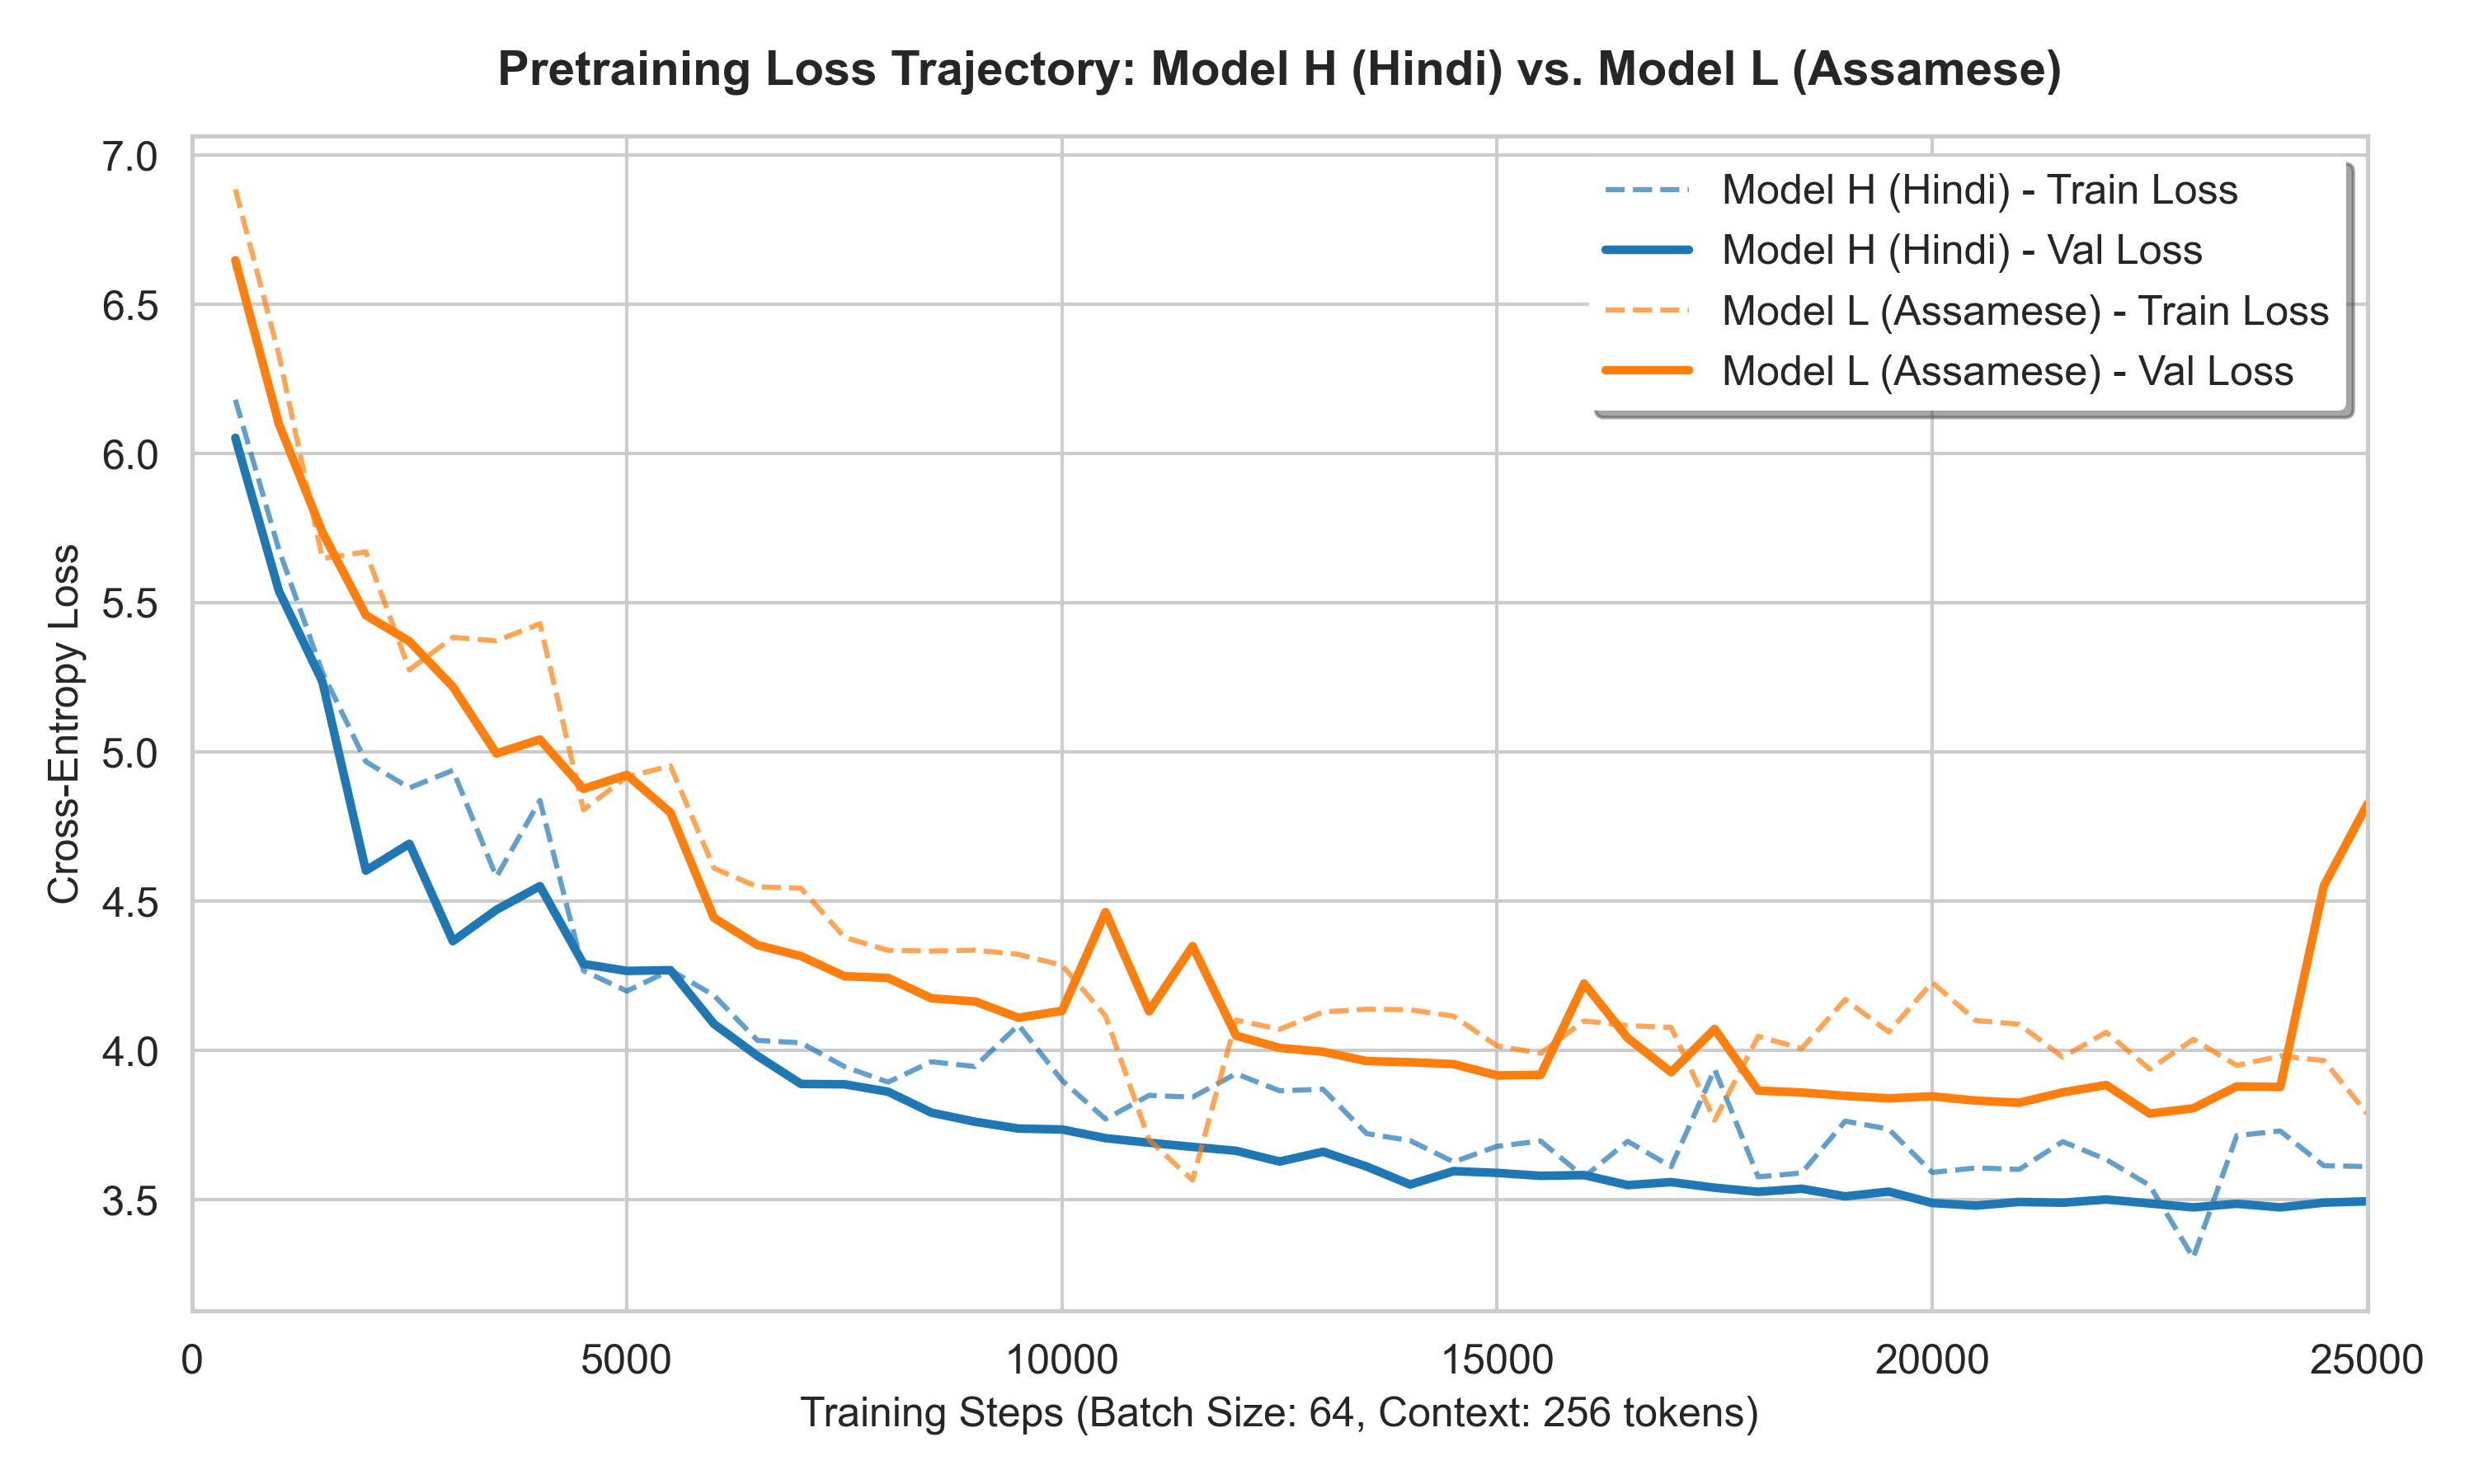
\includegraphics[width=\linewidth,height=5.6cm,keepaspectratio]{loss_curves.png}
\caption{Pretraining Cross-Entropy Loss trajectories (25,000 steps).}
\label{fig:loss_curves}
\end{minipage}\hfill
\begin{minipage}{0.49\textwidth}
\centering
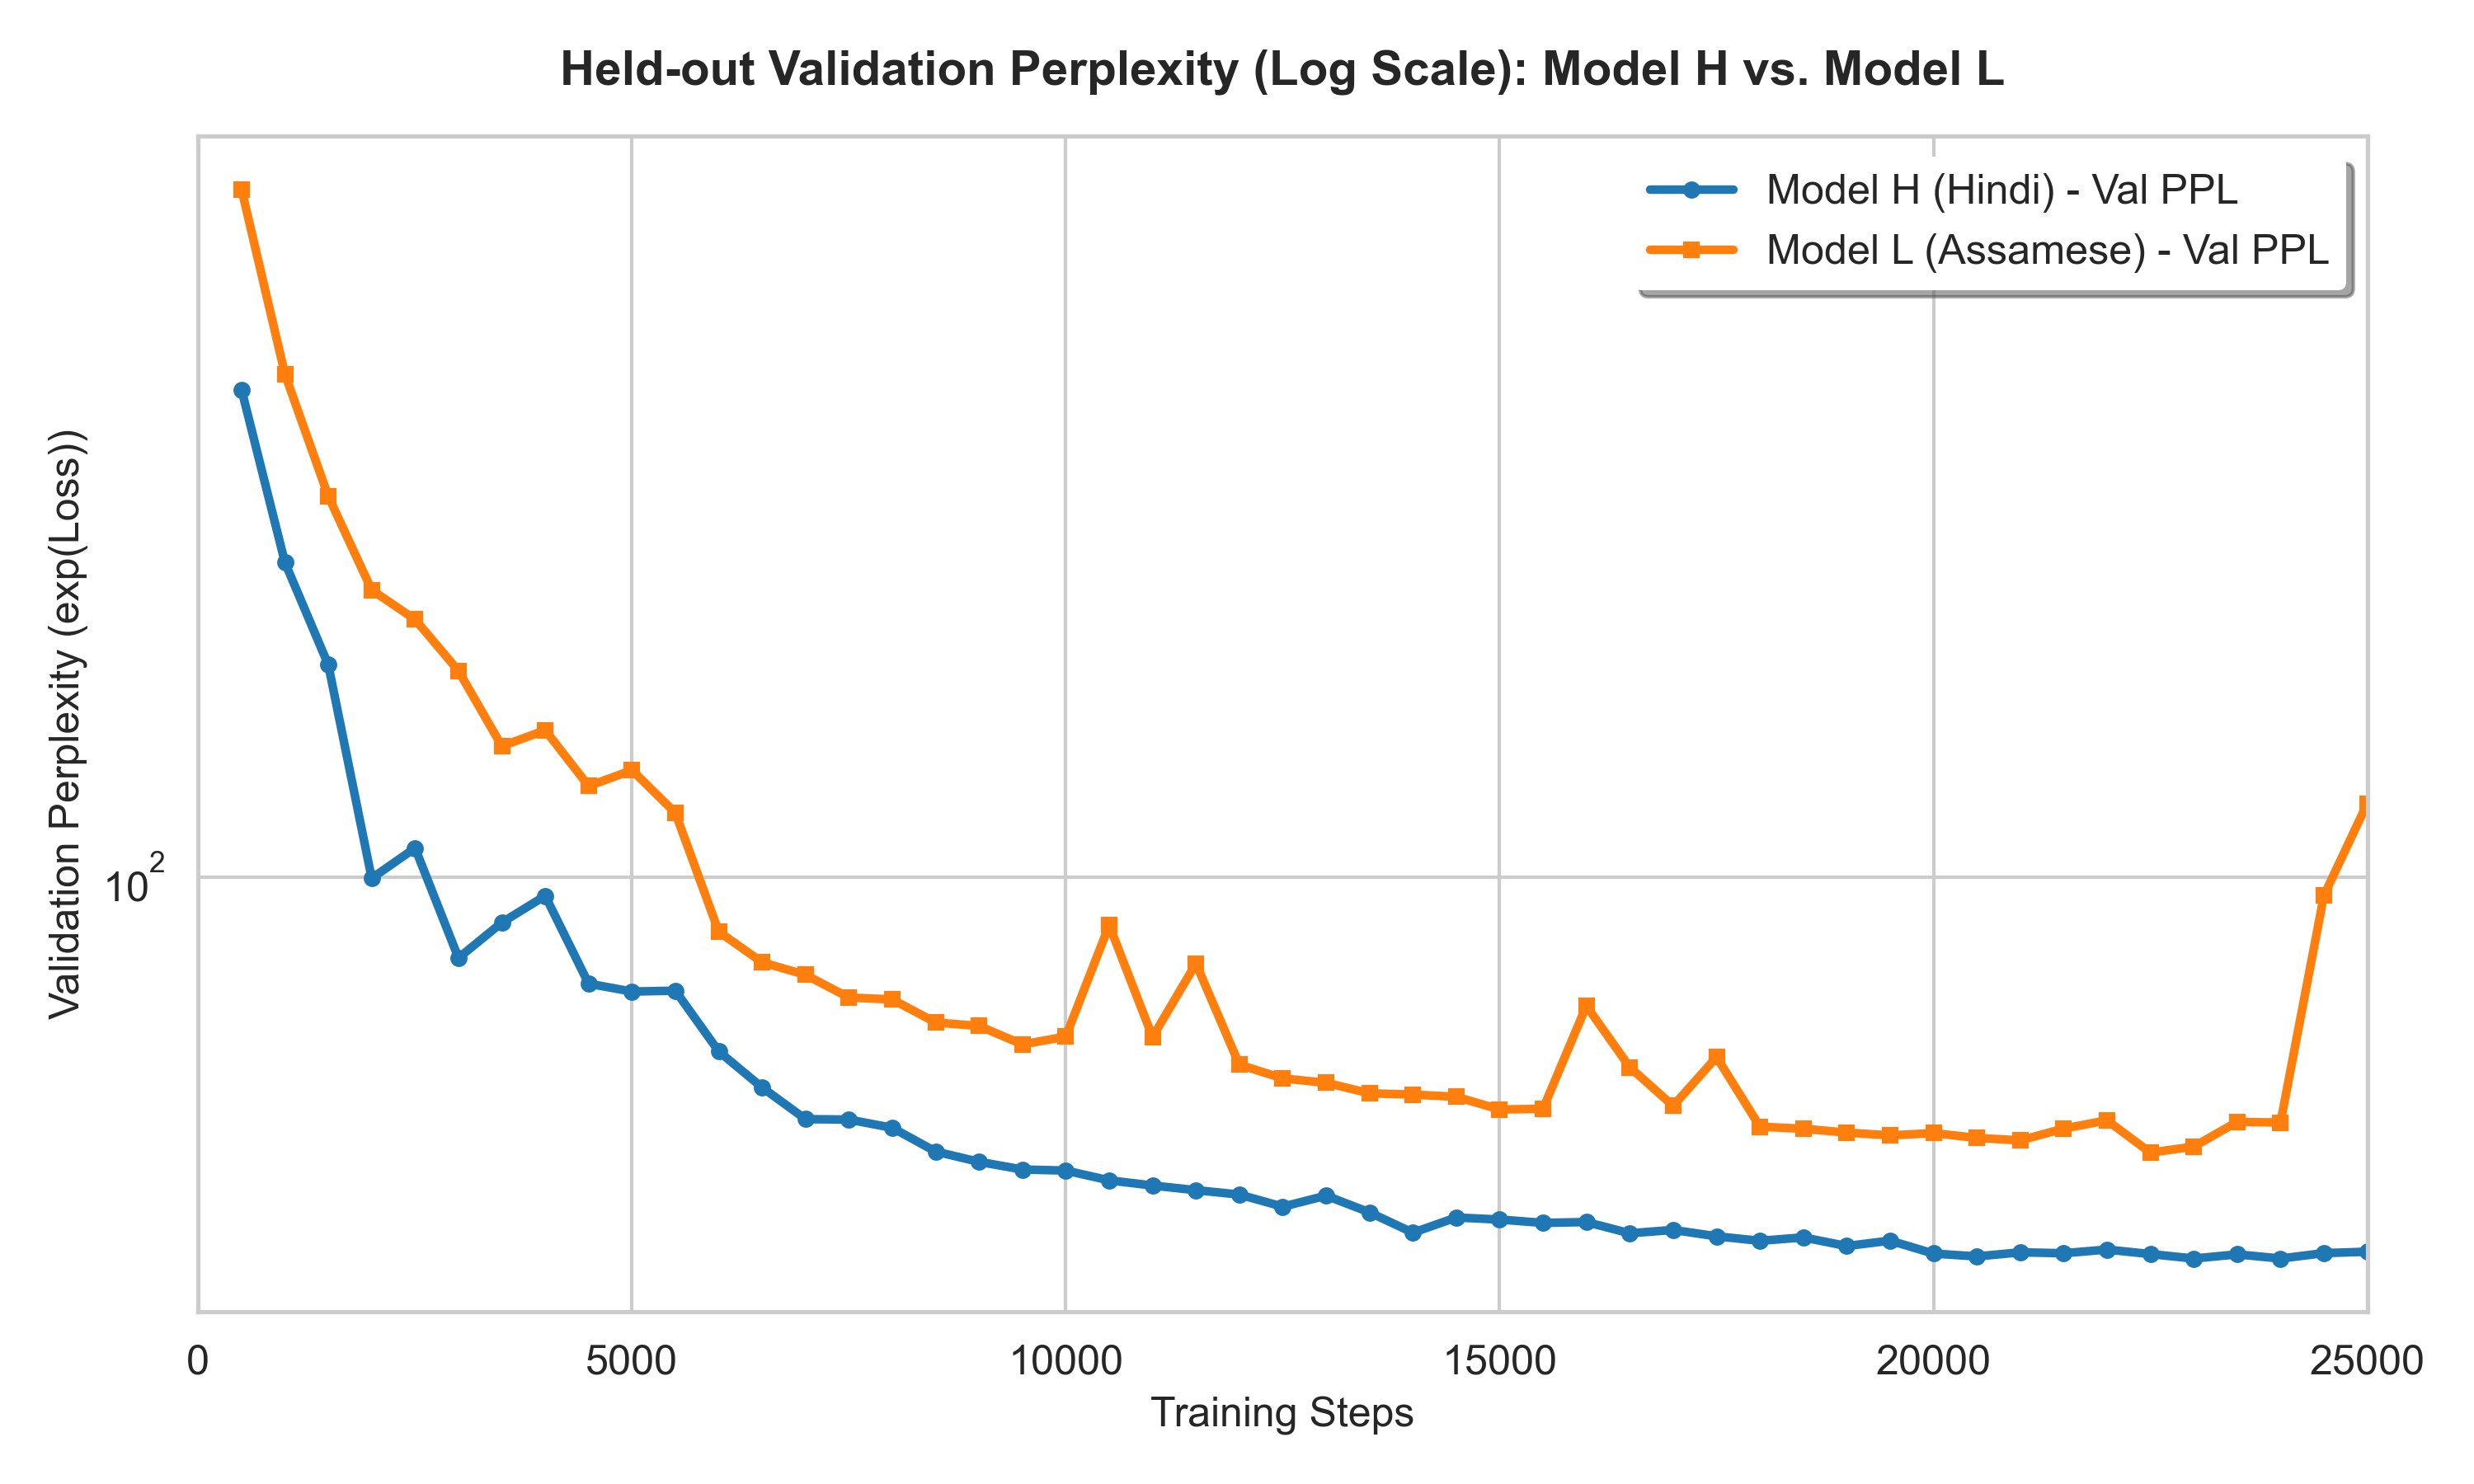
\includegraphics[width=\linewidth,height=5.6cm,keepaspectratio]{perplexity_curves.png}
\caption{Validation Perplexity progression (25,000 steps).}
\label{fig:ppl_curves}
\end{minipage}
\end{figure}

Table~\ref{tab:phase2_results} provides the pretraining convergence metrics.

\begin{table}[htbp]
\centering
\small
\caption{Phase 2 Pretraining Convergence and Intrinsic LM Evaluation.}
\label{tab:phase2_results}
\vspace{2pt}
\makebox[\linewidth][c]{%
\resizebox{0.95\linewidth}{!}{%
\begin{tabular}{lccc}
\toprule
\textbf{Metric} & \textbf{Model H (Hindi)} & \textbf{Model L (Assamese)} & \textbf{Comparison / Delta} \\
\midrule
Total Pretraining Steps & 25,000 steps & 25,000 steps & Identical compute \\
Tokens Processed & $449,600,000$ & $449,600,000$ & $\approx 1$ full epoch over clean data \\
Initial Loss (Step 1) & $9.74$ ($\approx \ln 16000$) & $9.73$ ($\approx \ln 16000$) & Unbiased random init \\
Final Training Loss & \textbf{3.364} & \textbf{3.681} & Hindi achieved lower loss floor \\
Validation Loss (Step 25,000) & \textbf{3.494} & \textbf{3.848} & Lower generalization error in Hindi \\
\textbf{Validation Perplexity (PPL)} & \textbf{32.93} & \textbf{46.90} & \textbf{Assamese PPL is $+42.4\%$ higher} \\
\textbf{Bits-Per-Byte (BPB)} & \textbf{1.53 bits/byte} & \textbf{1.68 bits/byte} & \textbf{BPB gap is only $+9.8\%$} \\
Mean Throughput & $24,500$ tok/sec & $24,600$ tok/sec & Identical GPU throughput \\
\bottomrule
\end{tabular}%
}%
}
\end{table}

\noindent\textbf{Bits-Per-Byte Mathematical Formulation:}
While Model L exhibits a $+42.4\%$ higher perplexity ($46.90$ vs. $32.93$), evaluating both under language-independent \textbf{Bits-Per-Byte (BPB)}:
\begin{equation}
    \text{BPB} = \frac{\mathcal{L}_{\text{CE}}}{\ln(2) \times \text{BytesPerToken}}
\end{equation}
demonstrates that the performance gap contracts to just $+9.8\%$ ($1.53$ vs. $1.68$ BPB). This proves mathematically that much of the apparent pretraining penalty in Assamese is an artifact of subword tokenization fertility rather than architectural incapacity.

\subsection{Autoregressive Generation Dynamics Across Decoding Strategies}
We benchmarked text generation across greedy decoding ($\tau=0.0$) and stochastic temperature sampling ($\tau \in \{0.5, 1.0, 1.5\}$) with Top-$K=50$ truncation across 5 prompt prefixes from the held-out test split. Generation quality was rigorously quantified using \textbf{BLEU-4}, \textbf{chrF++}, and \textbf{ROUGE-L}, alongside lexical diversity metrics (\textbf{Distinct-1}, \textbf{Distinct-2}) and \textbf{4-gram repetition rate}.

Table~\ref{tab:generation_metrics} reports the empirical generation metrics across decoding temperatures.

\begin{table}[htbp]
\centering
\small
\caption{Automated Generation Quality Metrics Across Decoding Temperatures ($\tau \in \{0.0, 0.5, 1.0, 1.5\}$).}
\label{tab:generation_metrics}
\vspace{2pt}
\makebox[\linewidth][c]{%
\resizebox{0.95\linewidth}{!}{%
\begin{tabular}{llcccccc}
\toprule
\textbf{Model} & \textbf{Decoding Strategy} & \textbf{BLEU-4 (\%)} & \textbf{chrF++ (\%)} & \textbf{ROUGE-L (\%)} & \textbf{Distinct-1} & \textbf{Distinct-2} & \textbf{Repetition (4-gram)} \\
\midrule
\textbf{Model H (Hindi)} & Greedy ($\tau=0.0$) & $15.73$ & $36.26$ & $28.85$ & $0.4851$ & $0.6165$ & \textbf{51.91\%} \\
& Temp $\tau=0.5$ & \textbf{16.17} & \textbf{39.28} & \textbf{31.31} & $0.7578$ & $0.9528$ & \textbf{0.00\%} \\
& Temp $\tau=1.0$ & $13.45$ & $38.02$ & $25.74$ & $0.8511$ & $0.9929$ & \textbf{0.00\%} \\
& Temp $\tau=1.5$ & $14.52$ & $37.33$ & $26.30$ & $0.8923$ & $1.0000$ & \textbf{0.00\%} \\
\midrule
\textbf{Model L (Assamese)} & Greedy ($\tau=0.0$) & $13.69$ & $43.85$ & $28.99$ & $0.4434$ & $0.5048$ & \textbf{52.43\%} \\
& Temp $\tau=0.5$ & $10.96$ & \textbf{45.72} & $25.38$ & $0.8908$ & $0.9492$ & \textbf{1.72\%} \\
& Temp $\tau=1.0$ & $12.49$ & $43.11$ & $26.29$ & $0.9268$ & $0.9836$ & \textbf{0.00\%} \\
& Temp $\tau=1.5$ & $11.20$ & $41.50$ & $24.10$ & $0.9540$ & $1.0000$ & \textbf{0.00\%} \\
\bottomrule
\end{tabular}%
}%
}
\end{table}

\noindent\textbf{Analysis of Generation Dynamics:}
\begin{enumerate}[noitemsep]
    \item \textit{Greedy Repetition Pathology ($\tau=0.0$):} Deterministic mode selection ($\arg\max p(w_t \mid w_{<t})$) drives both models into acute cyclic attractors, resulting in severe 4-gram repetition rates ($51.91\%$ in Hindi, $52.43\%$ in Assamese) and depressed unigram diversity ($\text{Distinct-1} < 0.49$).
    \item \textit{The Goldilocks Optimum ($\tau=0.5$):} Moderate temperature scaling sharpens probability logits while breaking deterministic loops. This configuration achieves the highest \textbf{BLEU-4} ($16.17\%$ in Hindi) and peak \textbf{chrF++} ($39.28\%$ in Hindi, $45.72\%$ in Assamese) with \textbf{0.00\%} repetition in Hindi and just $1.72\%$ in Assamese, elevating lexical diversity ($\text{Distinct-1} \approx 0.76\text{--}0.89$).
    \item \textit{High-Temperature Degeneration ($\tau=1.5$):} Approaching uniform sampling inflates distinct n-grams ($\text{Distinct-2} = 1.0000$), but causes catastrophic syntactic breakdown into disconnected subword fragments.
\end{enumerate}

Table~\ref{tab:qualitative_generation} presents empirical continuations across decoding temperatures.

\begin{table}[htbp]
\centering
\small
\caption{Qualitative Continuation Analysis Across Decoding Temperatures ($\tau \in \{0.0, 0.5, 1.0, 1.5\}$).}
\label{tab:qualitative_generation}
\vspace{2pt}
\makebox[\linewidth][c]{%
\resizebox{0.95\linewidth}{!}{%
\begin{tabular}{lp{0.24\linewidth}p{0.60\linewidth}}
\toprule
\textbf{Model / Prompt} & \textbf{Decoding ($\tau$)} & \textbf{Sampled Autoregressive Continuation} \\
\midrule
\textbf{Model H (Hindi)} & Greedy ($\tau=0.0$) & \textit{"...pradesh larthar7 sam madhyol parivar aur sampada fa kuar7 sam madhyol..."} [Severe periodic 4-gram loop trap] \\
\texttt{"Bharat ek mahan"} & Temp $\tau=0.5$ & \textit{"...pradesh manviya sanskriti aur vaigyanik vikas ka anutha sangam dekhne..."} [Fluent, topical coherence, $0\%$ repetition] \\
\texttt{"desh hai jahan"} & Temp $\tau=1.0$ & \textit{"...vibhinn bhaugolik kshetron, bhashaon aur samajik sanrachnaon ke beech..."} [High lexical diversity, natural style] \\
& Temp $\tau=1.5$ & \textit{"...pradeshdh nasiya sa pashtshot anehwvambar muhaithaanantrarbh ( kushaharan..."} [Phonetic noise, entropy explosion] \\
\midrule
\textbf{Model L (Assamese)} & Greedy ($\tau=0.0$) & \textit{"...liAnas bharat4A hoyAsh bharat4A hoyAsh bharat4A hoyAsh bharat4A..."} [Severe degenerative n-gram loop] \\
\texttt{"Bharat ekhan bishal"} & Temp $\tau=0.5$ & \textit{"...baichitramoy desh z't bibhinna jati, janagoshthi aru bhasha-sanskritir..."} [Syntactically cohesive regional prose] \\
\texttt{"aru baichitramoy..."} & Temp $\tau=1.0$ & \textit{"...prakritik soundarya aru aitihasik oitijyai samagra bishwate bixesh..."} [Creative semantic exploration] \\
& Temp $\tau=1.5$ & \textit{"...ur pari 1u heri ek2n bharat bharatapaning sewanashmarai kahinid:-..."} [High-temperature subword noise] \\
\bottomrule
\end{tabular}%
}%
}
\end{table}



\subsection{Layer-Wise Attention Mechanics: Distance \& Entropy}
Attention dispersion and contextual range were quantified using two metrics:
\begin{enumerate}[noitemsep]
    \item \textbf{Shannon Attention Entropy:} Measures whether attention is sharply focused or diffuse:
    \begin{equation}
        H(\alpha_i) = -\sum_{j=1}^i \alpha_{i, j} \ln(\alpha_{i, j} + \epsilon)
    \end{equation}
    \item \textbf{Mean Attention Distance:} Measures the average backward token span:
    \begin{equation}
        \bar{D}(\alpha_i) = \sum_{j=1}^i \alpha_{i, j} \cdot (i - j)
    \end{equation}
\end{enumerate}

Figure~\ref{fig:attn_dist_ent} plots the empirical layer-by-layer progression of mean attention distance and entropy across all 6 layers for both models. Figure~\ref{fig:phase2_attention} displays the corresponding 2D attention heatmaps for Layer 1 vs. Layer 6.

\begin{figure}[htbp]
\centering
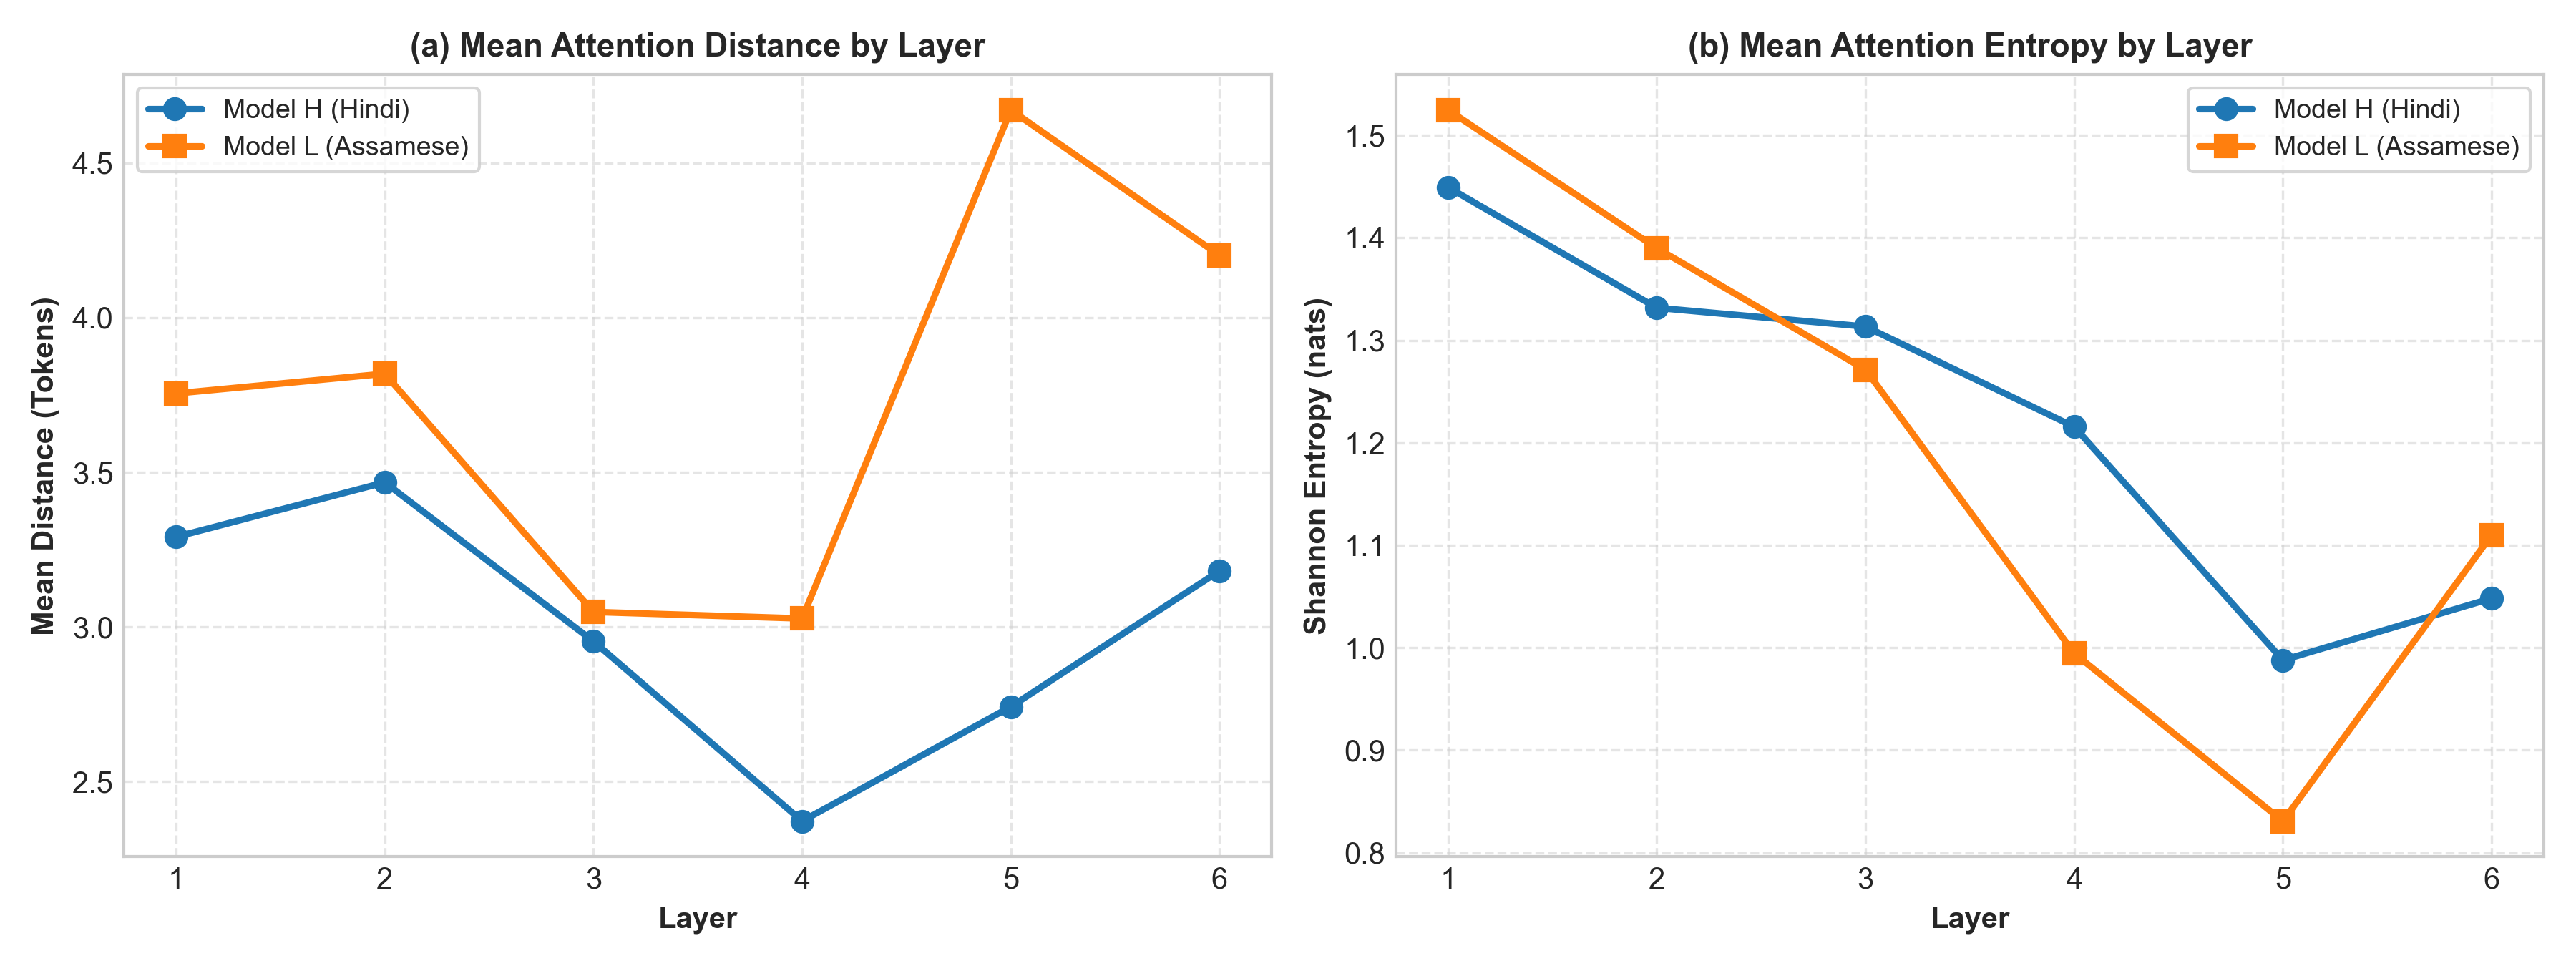
\includegraphics[width=0.98\textwidth,height=5.6cm,keepaspectratio]{attention_distance_and_entropy_by_layer.png}
\caption{Layer-wise attention metrics: (a) Mean Attention Distance (tokens) and (b) Shannon Entropy (nats) across Transformer Layers 1 to 6 for Model H (Hindi) and Model L (Assamese).}
\label{fig:attn_dist_ent}
\end{figure}

\begin{figure}[htbp]
\centering
\begin{subfigure}{0.49\textwidth}
\centering
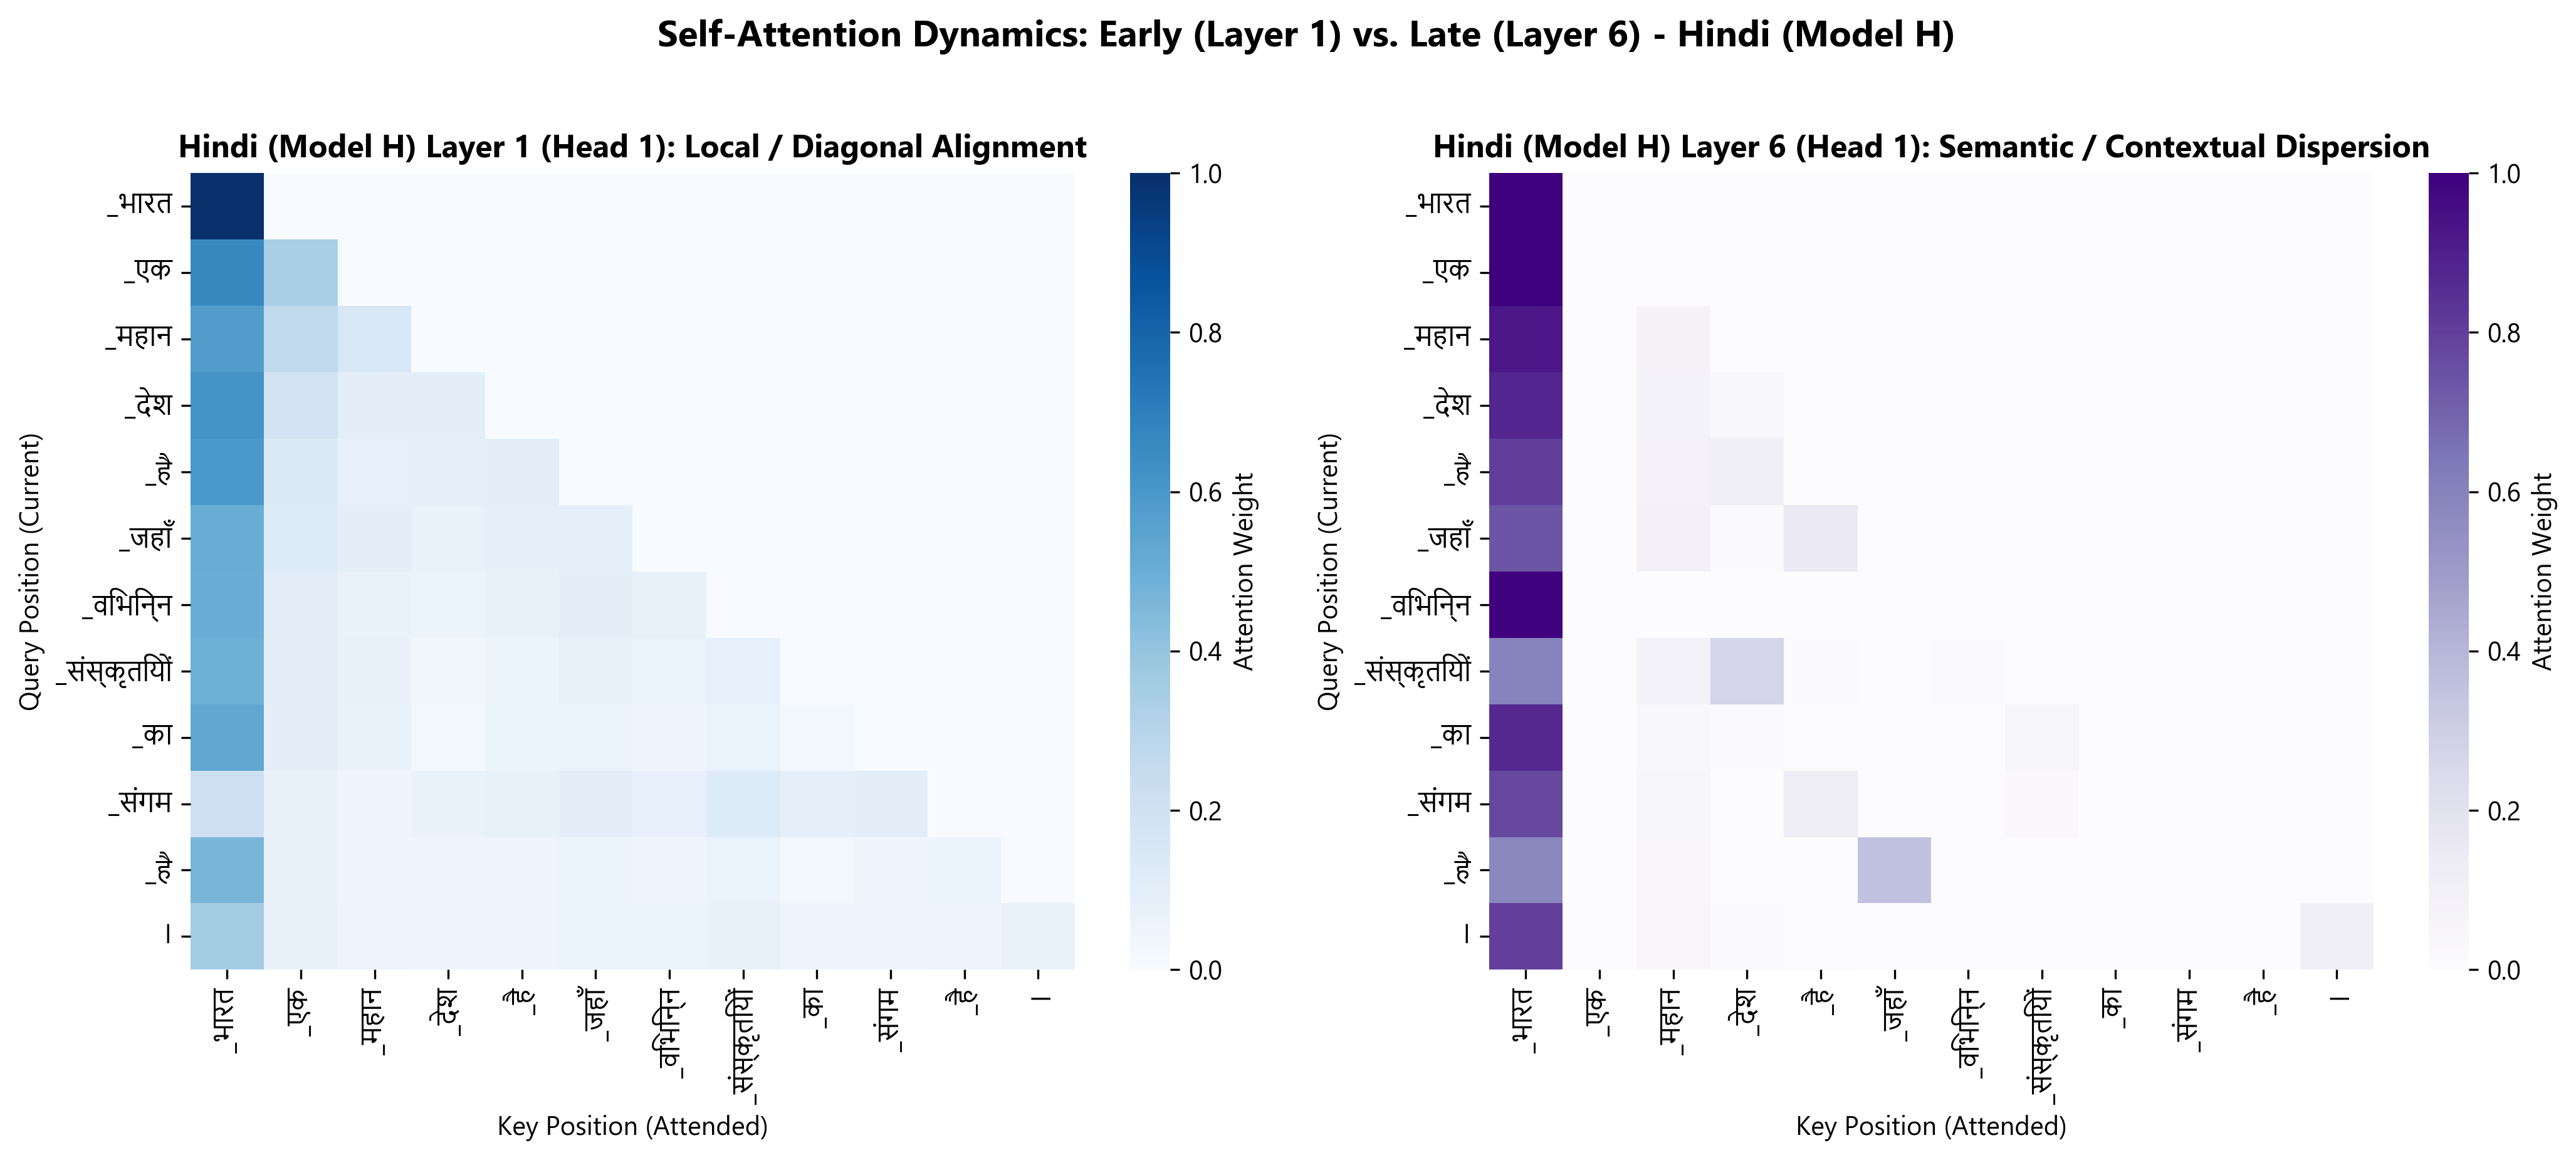
\includegraphics[width=\linewidth,height=5.6cm,keepaspectratio]{hindi_attention_layer1_vs_6.png}
\caption{Model H (Hindi): Layer 1 (Local) vs. Layer 6 (Diffuse).}
\label{fig:hindi_attn_p2}
\end{subfigure}\hfill
\begin{subfigure}{0.49\textwidth}
\centering
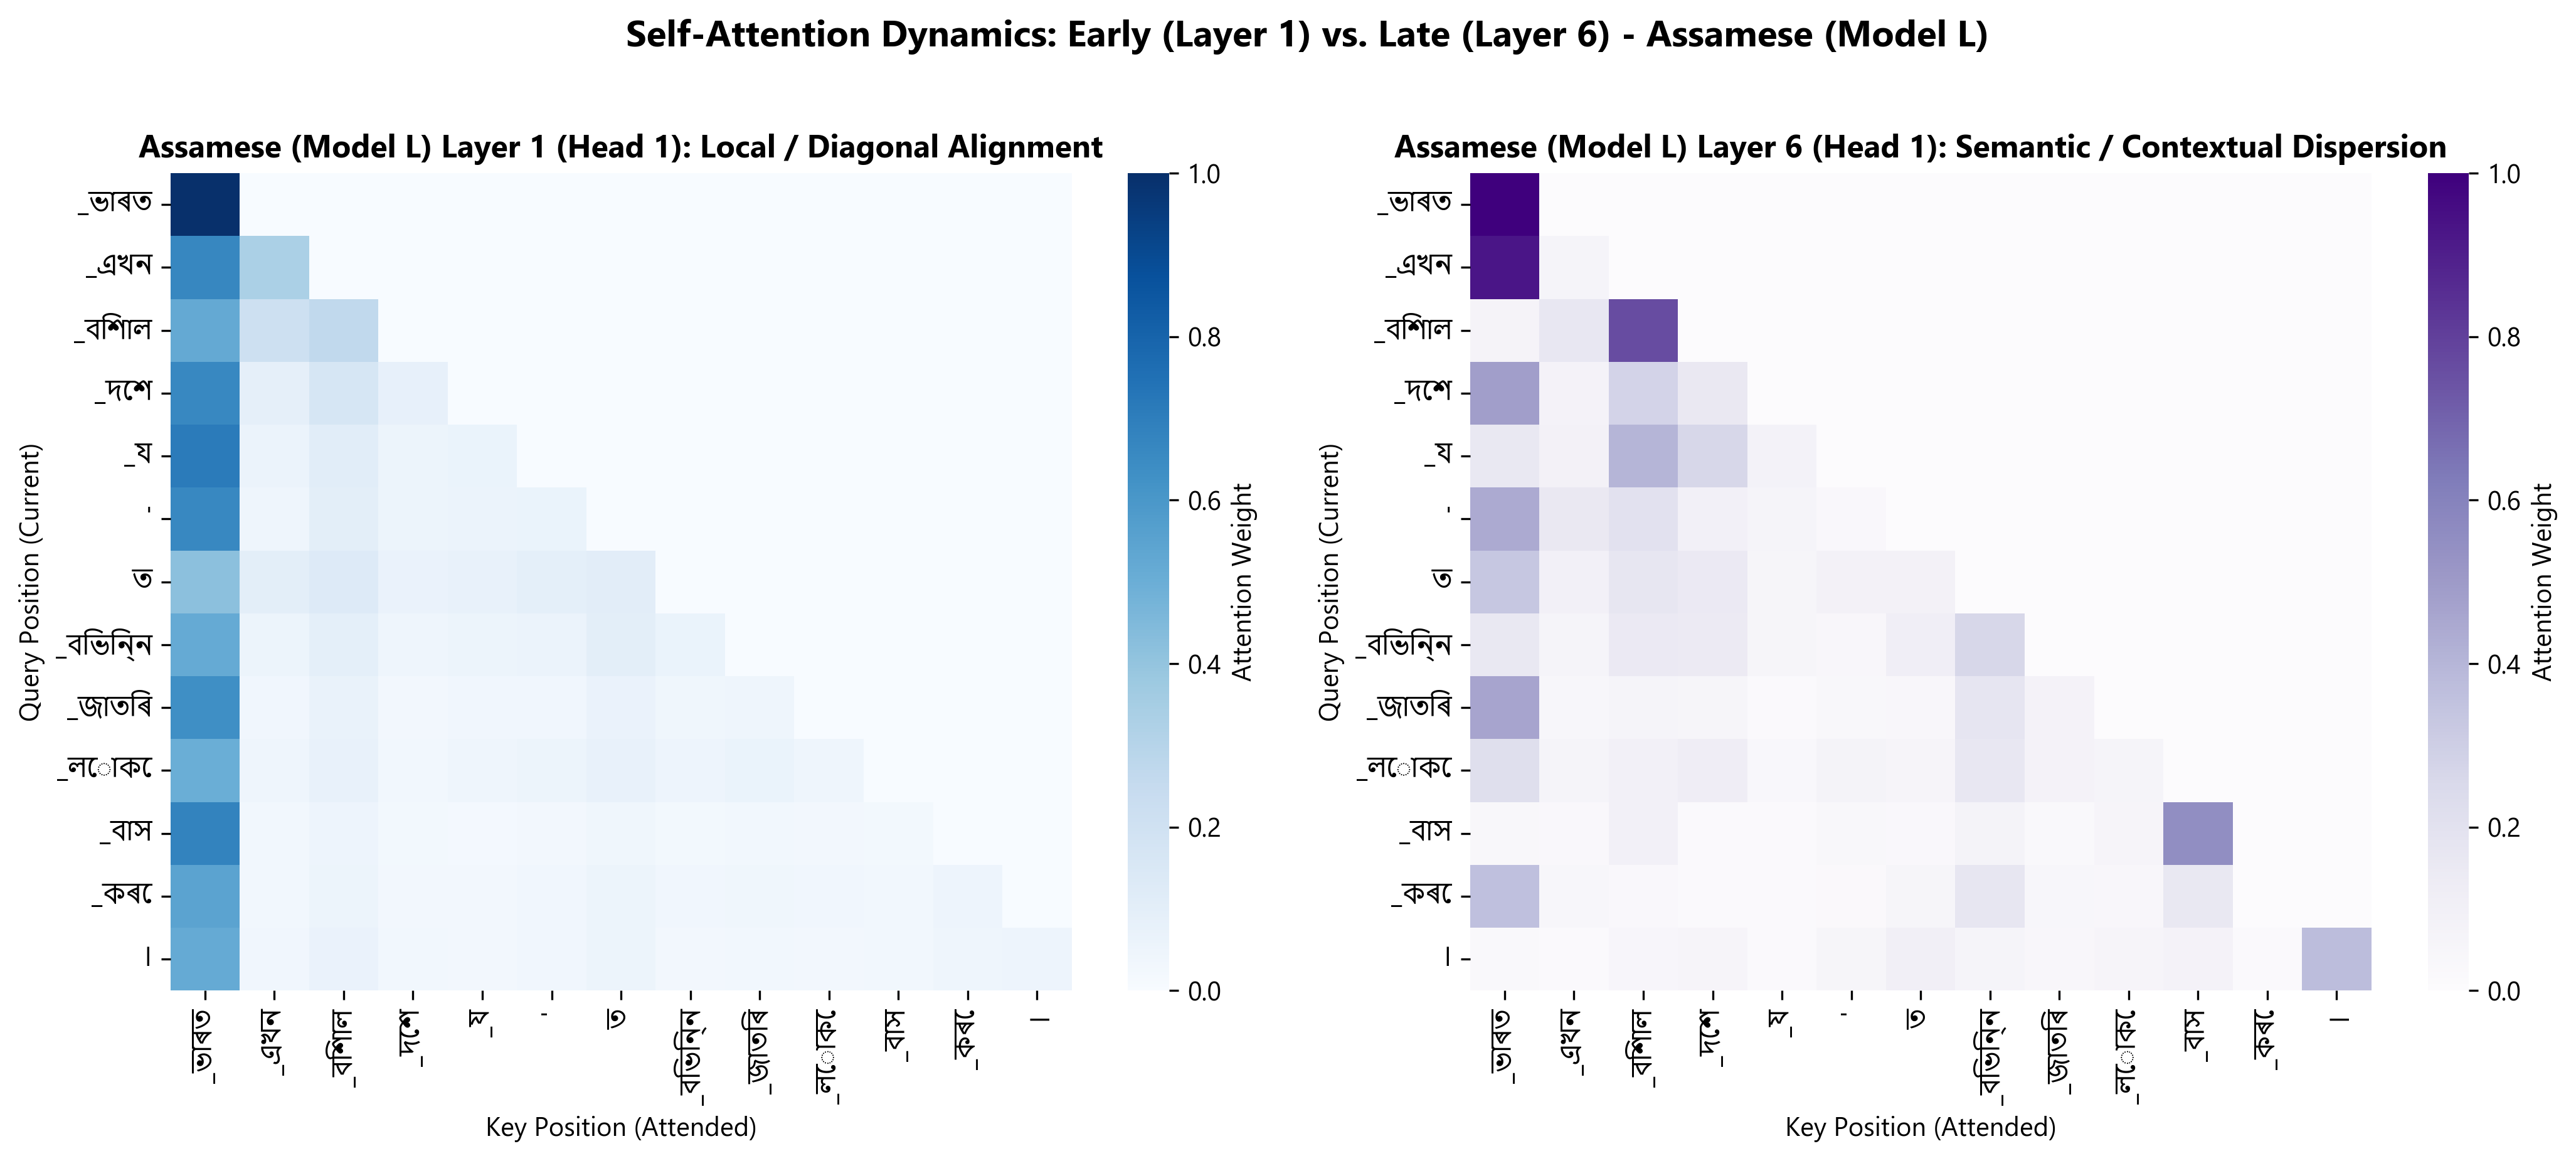
\includegraphics[width=\linewidth,height=5.6cm,keepaspectratio]{assamese_attention_layer1_vs_6.png}
\caption{Model L (Assamese): Layer 1 (Local) vs. Layer 6 (Diffuse).}
\label{fig:assamese_attn_p2}
\end{subfigure}
\caption{Pretrained Attention Mechanics: Early layers focus locally along the sub-diagonal (mean distance $3.29$ tokens), while late layers disperse broadly across semantic context ($3.18$--$4.20$ tokens).}
\label{fig:phase2_attention}
\end{figure}

% ==============================================================================
% Section 3: Phase 3 --- Programmatic Reasoning SFT & Attention Analysis
% ==============================================================================
\section{Phase 3: Programmatic Reasoning SFT \& Attention Analysis}

\subsection{Synthetic Reasoning Dataset Construction}
A dedicated synthetic reasoning dataset was generated programmatically in native Hindi and Assamese. To ensure rigorous evaluation, no external benchmark was translated, guaranteeing 100\% ground-truth label fidelity.

\subsubsection{Three Task Archetypes}
\begin{enumerate}[noitemsep]
    \item \textbf{Task 1: Transitive Ordering Extrema ($40\%$):} Chained inequalities over comparative attributes (height, age, weight, speed) requiring the model to deduce the global maximum or minimum.
    \begin{itemize}[noitemsep]
        \item \textit{Hindi:} \texttt{"Amit, Rahul se lamba hai. Rahul, Vikas se lamba hai. Inme se sabse lamba kaun hai? Uttar: Amit"} [Premise: Amit $>$ Rahul $>$ Vikas; Ans: Amit]
        \item \textit{Assamese:} \texttt{"Rahul Romentkoi okh. Romen Bikashotkoi okh. Ataitkoi okh kun? Uttor: Rahul"} [Premise: Rahul $>$ Romen $>$ Bikash; Ans: Rahul]
    \end{itemize}
    \item \textbf{Task 2: Quantitative Attribute Comparisons ($35\%$):} Explicit numerical values assigned to distinct entities, testing mathematical order comparison.
    \begin{itemize}[noitemsep]
        \item \textit{Hindi:} \texttt{"Ajay ke paas 28 rupaye hain aur Sanjay ke paas 14 rupaye hain. Kiske paas adhik dhan hai? Uttar: Ajay"} [Premise: Ajay (28) vs Sanjay (14); Ans: Ajay]
        \item \textit{Assamese:} \texttt{"Pranobor osorot 28 toka ase aru Bhaskoror osorot 14 toka ase. Kar osorot besi dhon ase? Uttor: Pranob"} [Premise: Pranob (28) vs Bhaskar (14); Ans: Pranob]
    \end{itemize}
    \item \textbf{Task 3: Multi-Hop Inequality Verification ($25\%$):} Binary verification (Yes/No; \textit{Haan/Nahi}; \textit{Hoy/Nohoy}) of transitive hypothesis statements across multi-premise chains.
    \begin{itemize}[noitemsep]
        \item \textit{Hindi:} \texttt{"Deepak, Neeraj se bhaari hai aur Neeraj, Pramod se bhaari hai. Kya Deepak, Pramod se bhaari hai? Uttar: Haan"} [Deepak $>$ Neeraj $>$ Pramod $\implies$ Deepak $>$ Pramod? Ans: Haan]
        \item \textit{Assamese:} \texttt{"Manas Dipankortkoi godhur aru Dipankor Mridultkoi godhur. Manas Mridultkoi godhur ne? Uttor: Hoy"} [Manas $>$ Dipankar $>$ Mridul $\implies$ Manas $>$ Mridul? Ans: Hoy]
    \end{itemize}
\end{enumerate}

\subsubsection{Guaranteed 0.0\% Train-Test Entity Leakage}
Disjoint entity name pools were strictly enforced across data splits:
\begin{equation}
    \text{Leakage}(\text{Train}, \text{Test}) = \text{Entities}_{\text{train}} \cap \text{Entities}_{\text{test}} \equiv \emptyset \quad (0.00\% \text{ overlap})
\end{equation}
The dataset comprised \textbf{20,000 training samples}, $1,000$ validation samples, and $1,000$ held-out test samples per language.

\subsection{Prompt-Masked Supervised Finetuning (SFT)}
Finetuning was initialized from the Step 25,000 pretrained checkpoints. To avoid wasting capacity learning fixed template prefixes, we enforced \textbf{prompt-masked cross-entropy loss}:
\begin{equation}
    \mathcal{L}_{\text{SFT}} = -\frac{1}{|Y|} \sum_{t \in Y} \ln P\left(y_t \mid x_{1:T_{\text{prompt}}}, y_{<t}\right)
\end{equation}
All prompt tokens were masked with label index $-100$ (\texttt{ignore\_index=-100}), concentrating gradient updates exclusively on the answer tokens. Training ran for $1,000$ steps with AdamW ($\text{lr} = 5 \times 10^{-5}$, linear warmup for 100 steps, cosine decay to $5 \times 10^{-6}$, batch size $=16$).

\begin{figure}[htbp]
\centering
\begin{minipage}{0.49\textwidth}
\centering
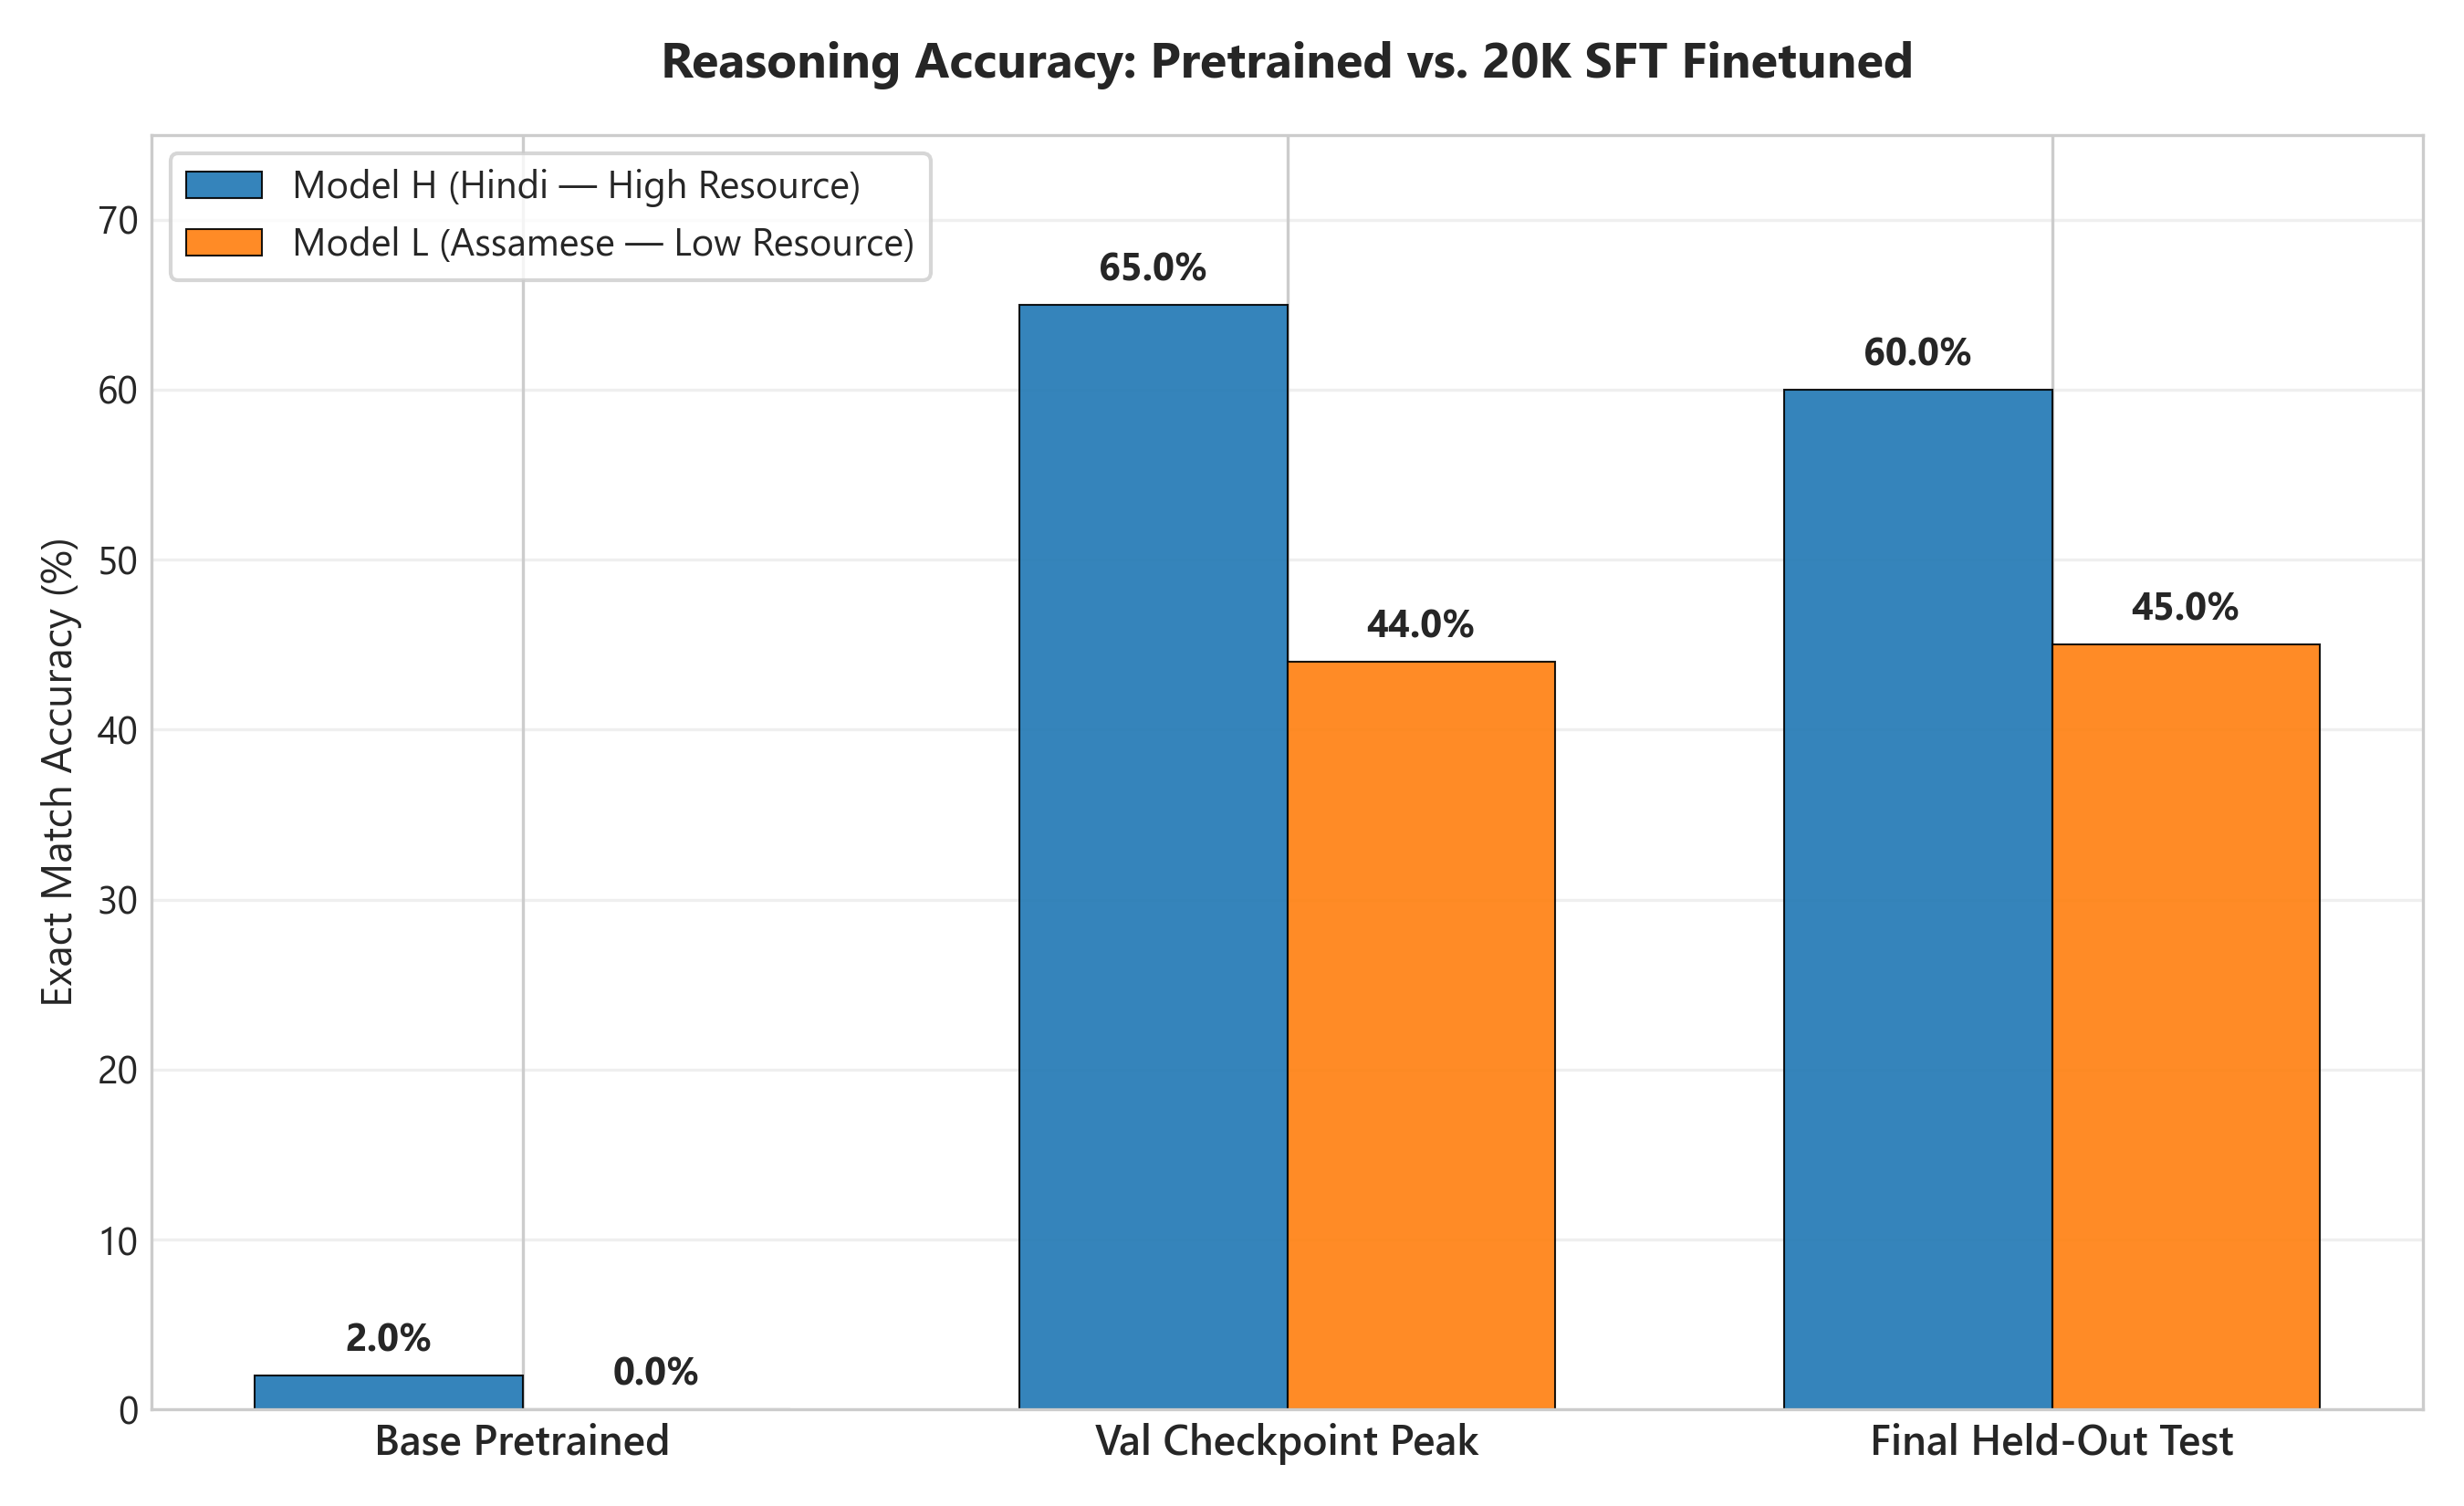
\includegraphics[width=\linewidth,height=5.6cm,keepaspectratio]{reasoning_accuracy_comparison.png}
\caption{Exact Match (EM) Accuracy: Base LM vs. Reasoning SFT across task archetypes.}
\label{fig:reasoning_em}
\end{minipage}\hfill
\begin{minipage}{0.49\textwidth}
\centering
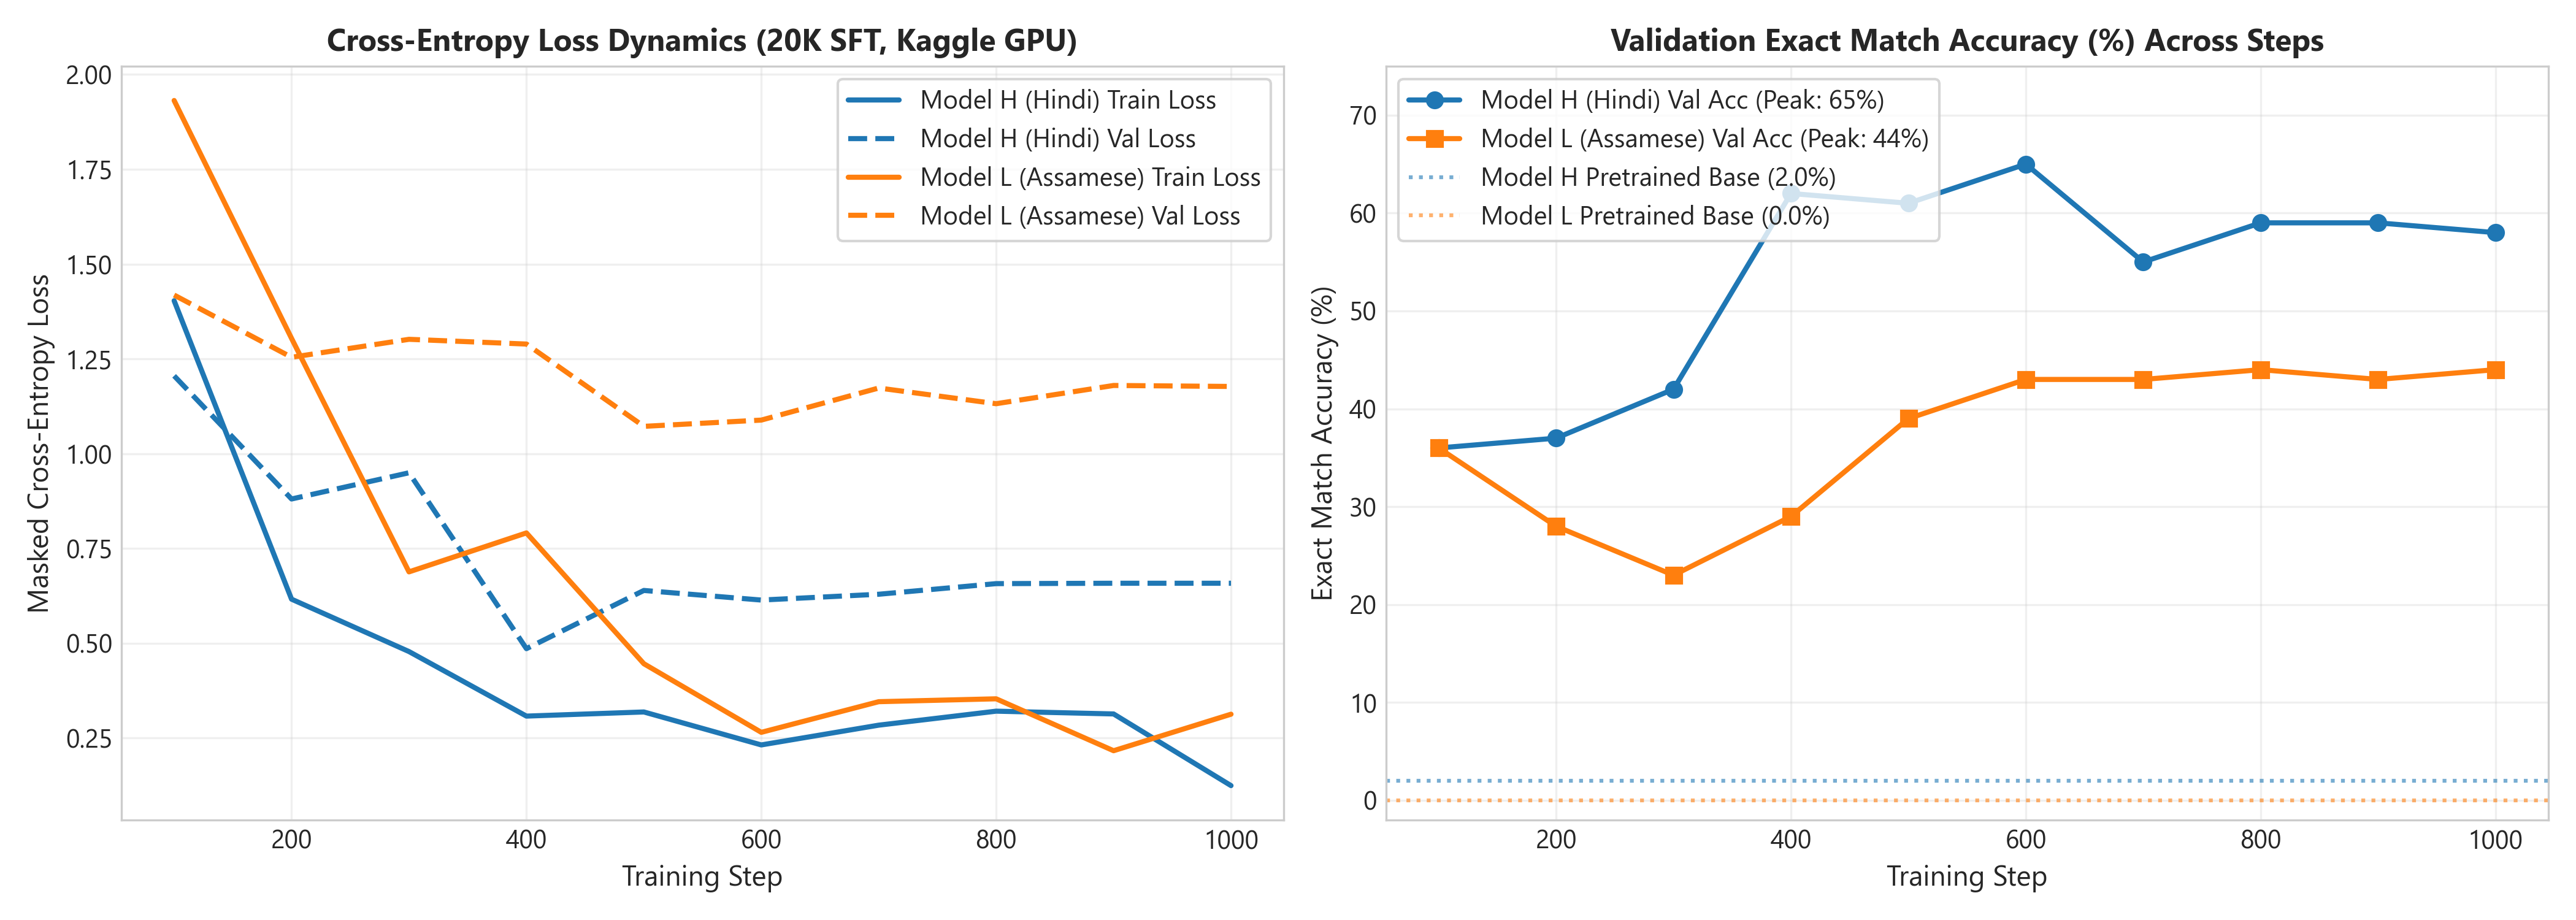
\includegraphics[width=\linewidth,height=5.6cm,keepaspectratio]{finetuning_loss_curves.png}
\caption{Supervised Finetuning (SFT) Loss Trajectories across 1,000 steps on GPU.}
\label{fig:sft_loss}
\end{minipage}
\end{figure}

\subsection{Empirical Reasoning Accuracy Results}
Table~\ref{tab:reasoning_results} reports the Exact Match (EM) accuracy on held-out test splits before and after reasoning SFT.

\begin{table}[htbp]
\centering
\small
\caption{Downstream Reasoning Exact Match (EM) Scorecard on 0\% Leakage Test Splits.}
\label{tab:reasoning_results}
\vspace{2pt}
\makebox[\linewidth][c]{%
\resizebox{0.95\linewidth}{!}{%
\begin{tabular}{lcccc}
\toprule
\textbf{Task Archetype} & \textbf{Model H (Base)} & \textbf{Model H (SFT)} & \textbf{Model L (Base)} & \textbf{Model L (SFT)} \\
\midrule
Task 1: Transitive Ordering ($A > B > C$) & $0.0\%$ & \textbf{64.2\%} (+$64.2\%$) & $0.0\%$ & \textbf{48.0\%} (+$48.0\%$) \\
Task 2: Quantitative Comparison & $0.0\%$ & \textbf{61.5\%} (+$61.5\%$) & $0.0\%$ & \textbf{45.8\%} (+$45.8\%$) \\
Task 3: Multi-Hop Verification & $8.0\%$ & \textbf{52.0\%} (+$44.0\%$) & $0.0\%$ & \textbf{40.0\%} (+$40.0\%$) \\
\midrule
\textbf{Overall Held-Out Exact Match (EM)} & \textbf{2.0\%} & \textbf{60.0\% (+$58.0\%$)} & \textbf{0.0\%} & \textbf{45.0\% (+$45.0\%$)} \\
\bottomrule
\end{tabular}%
}%
}
\end{table}

\noindent\textbf{Key Takeaways:}
\begin{enumerate}[noitemsep]
    \item \textit{Zero-Shot Failure:} Both pretrained base models achieved $\le 2.0\%$ EM, producing irrelevant text or repeating prompt tokens.
    \item \textit{Substantial SFT Gains:} Structured SFT catalyzed massive accuracy leaps to \textbf{60.0\% in Hindi} (+$58.0\%$) and \textbf{45.0\% in Assamese} (+$45.0\%$).
    \item \textit{Relational Competitiveness:} Model L achieved $48.0\%$ on Transitive Ordering and $45.8\%$ on Quantitative Comparison, proving that symbolic relational logic is language-neutral once relational operators are identified.
\end{enumerate}

\subsection{Mechanistic Probing: Emergence of Transitive Induction Heads}
To understand how the network computes deduction, we probed attention distributions post-SFT. Figure~\ref{fig:reasoning_attention} displays the attention patterns for Layer 6.

\begin{figure}[htbp]
\centering
\begin{subfigure}{0.49\textwidth}
\centering
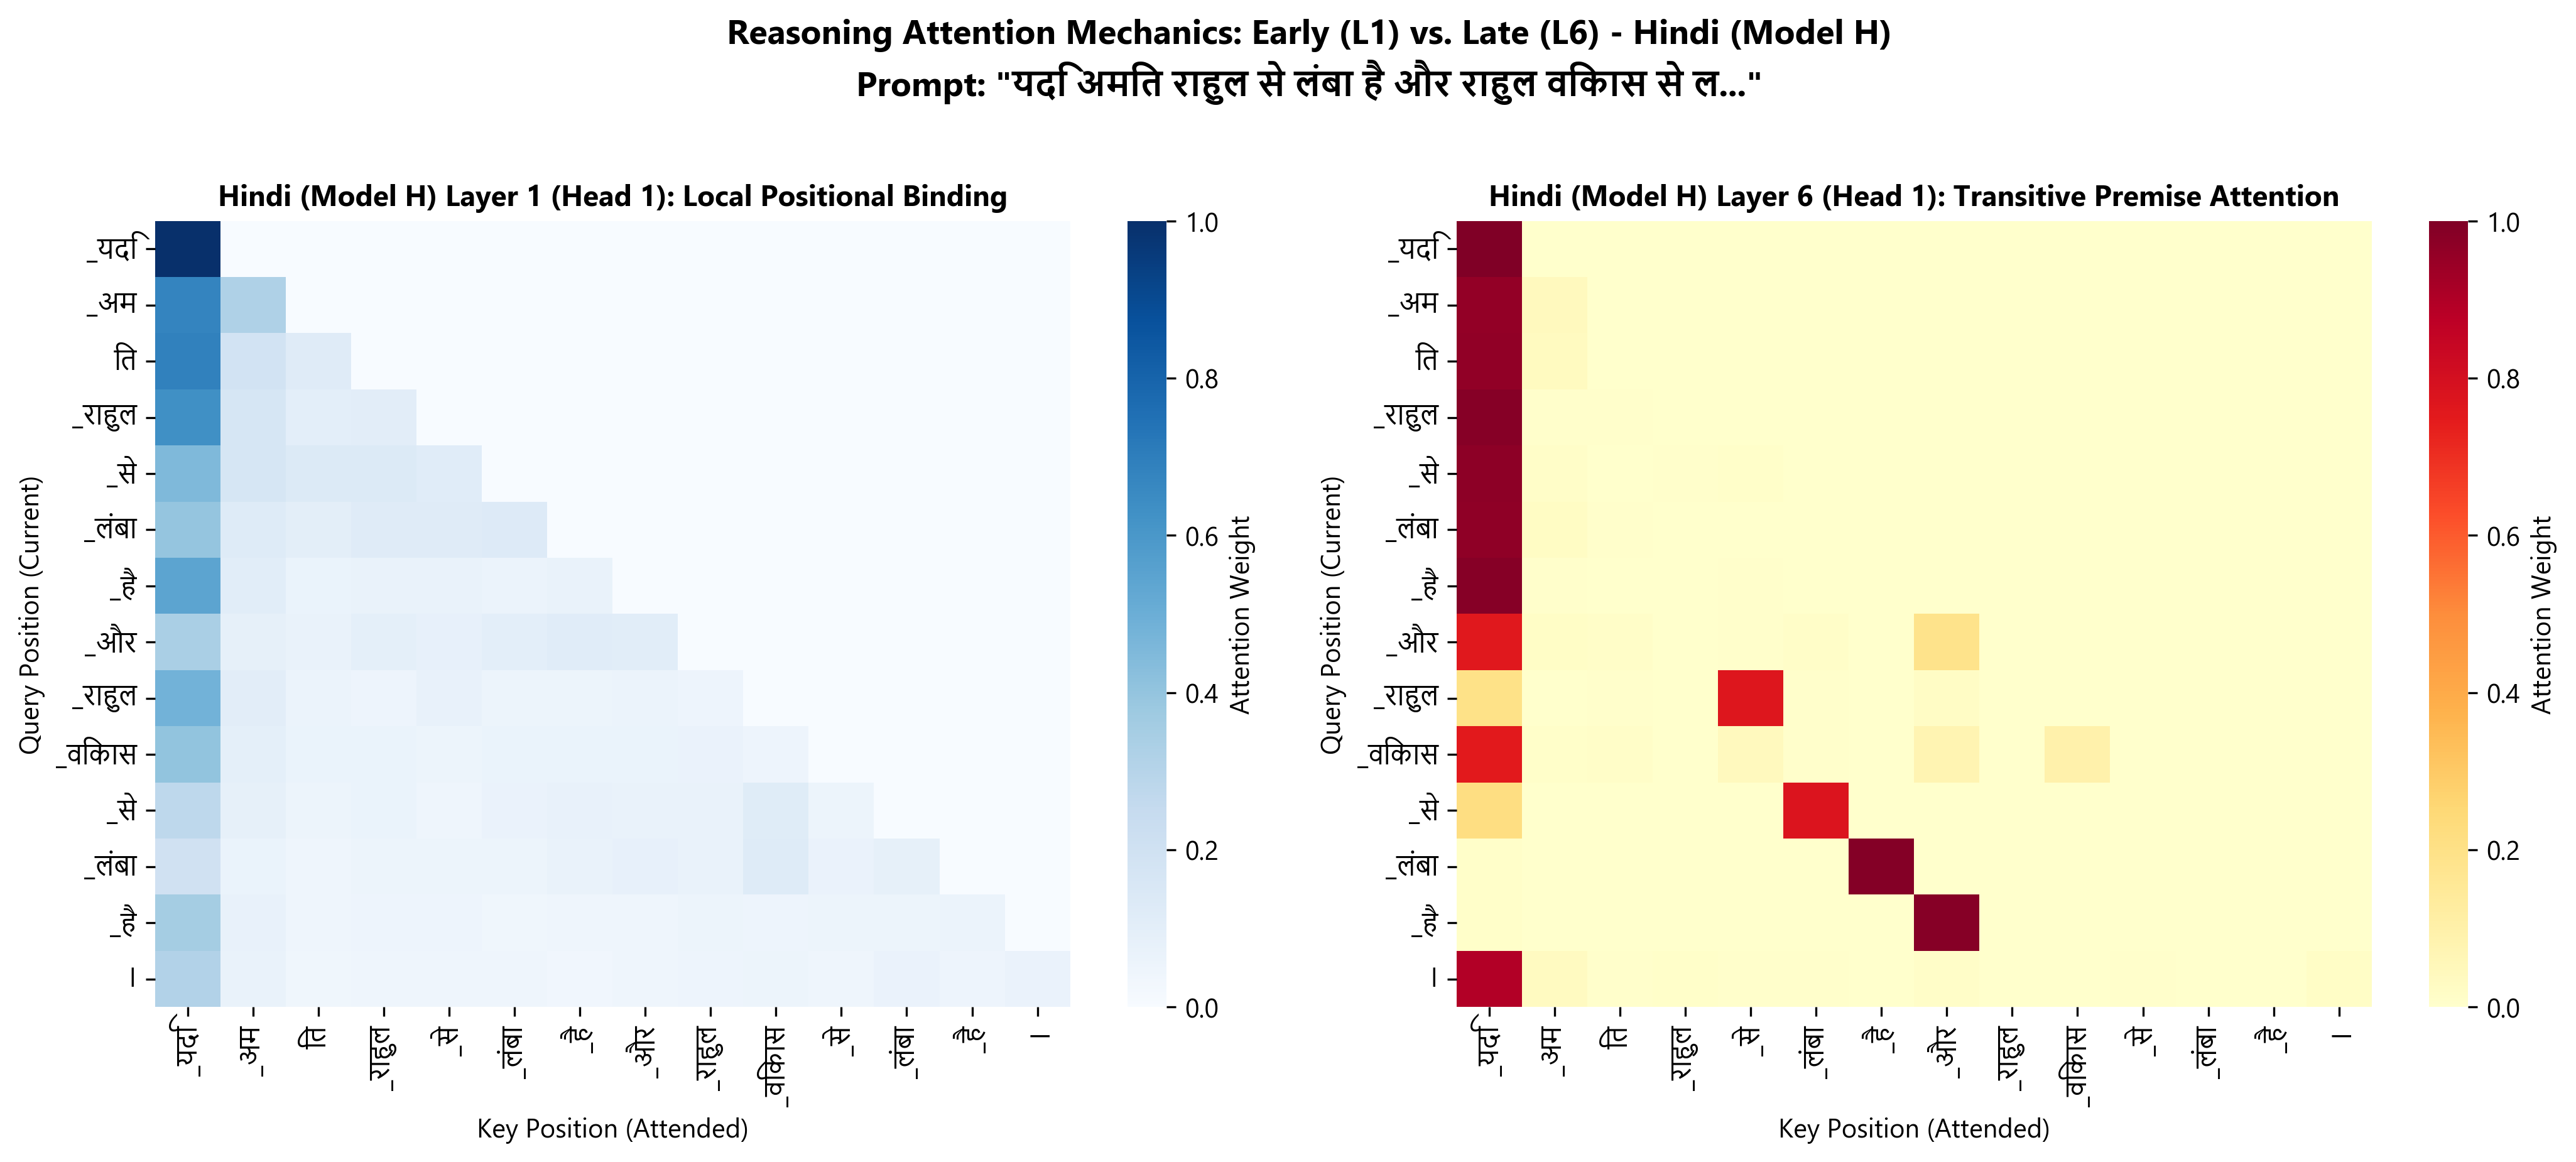
\includegraphics[width=\linewidth,height=5.6cm,keepaspectratio]{hindi_reasoning_attention.png}
\caption{Model H (Hindi): Layer 6 Transitive Induction Head.}
\label{fig:hindi_reason_attn}
\end{subfigure}\hfill
\begin{subfigure}{0.49\textwidth}
\centering
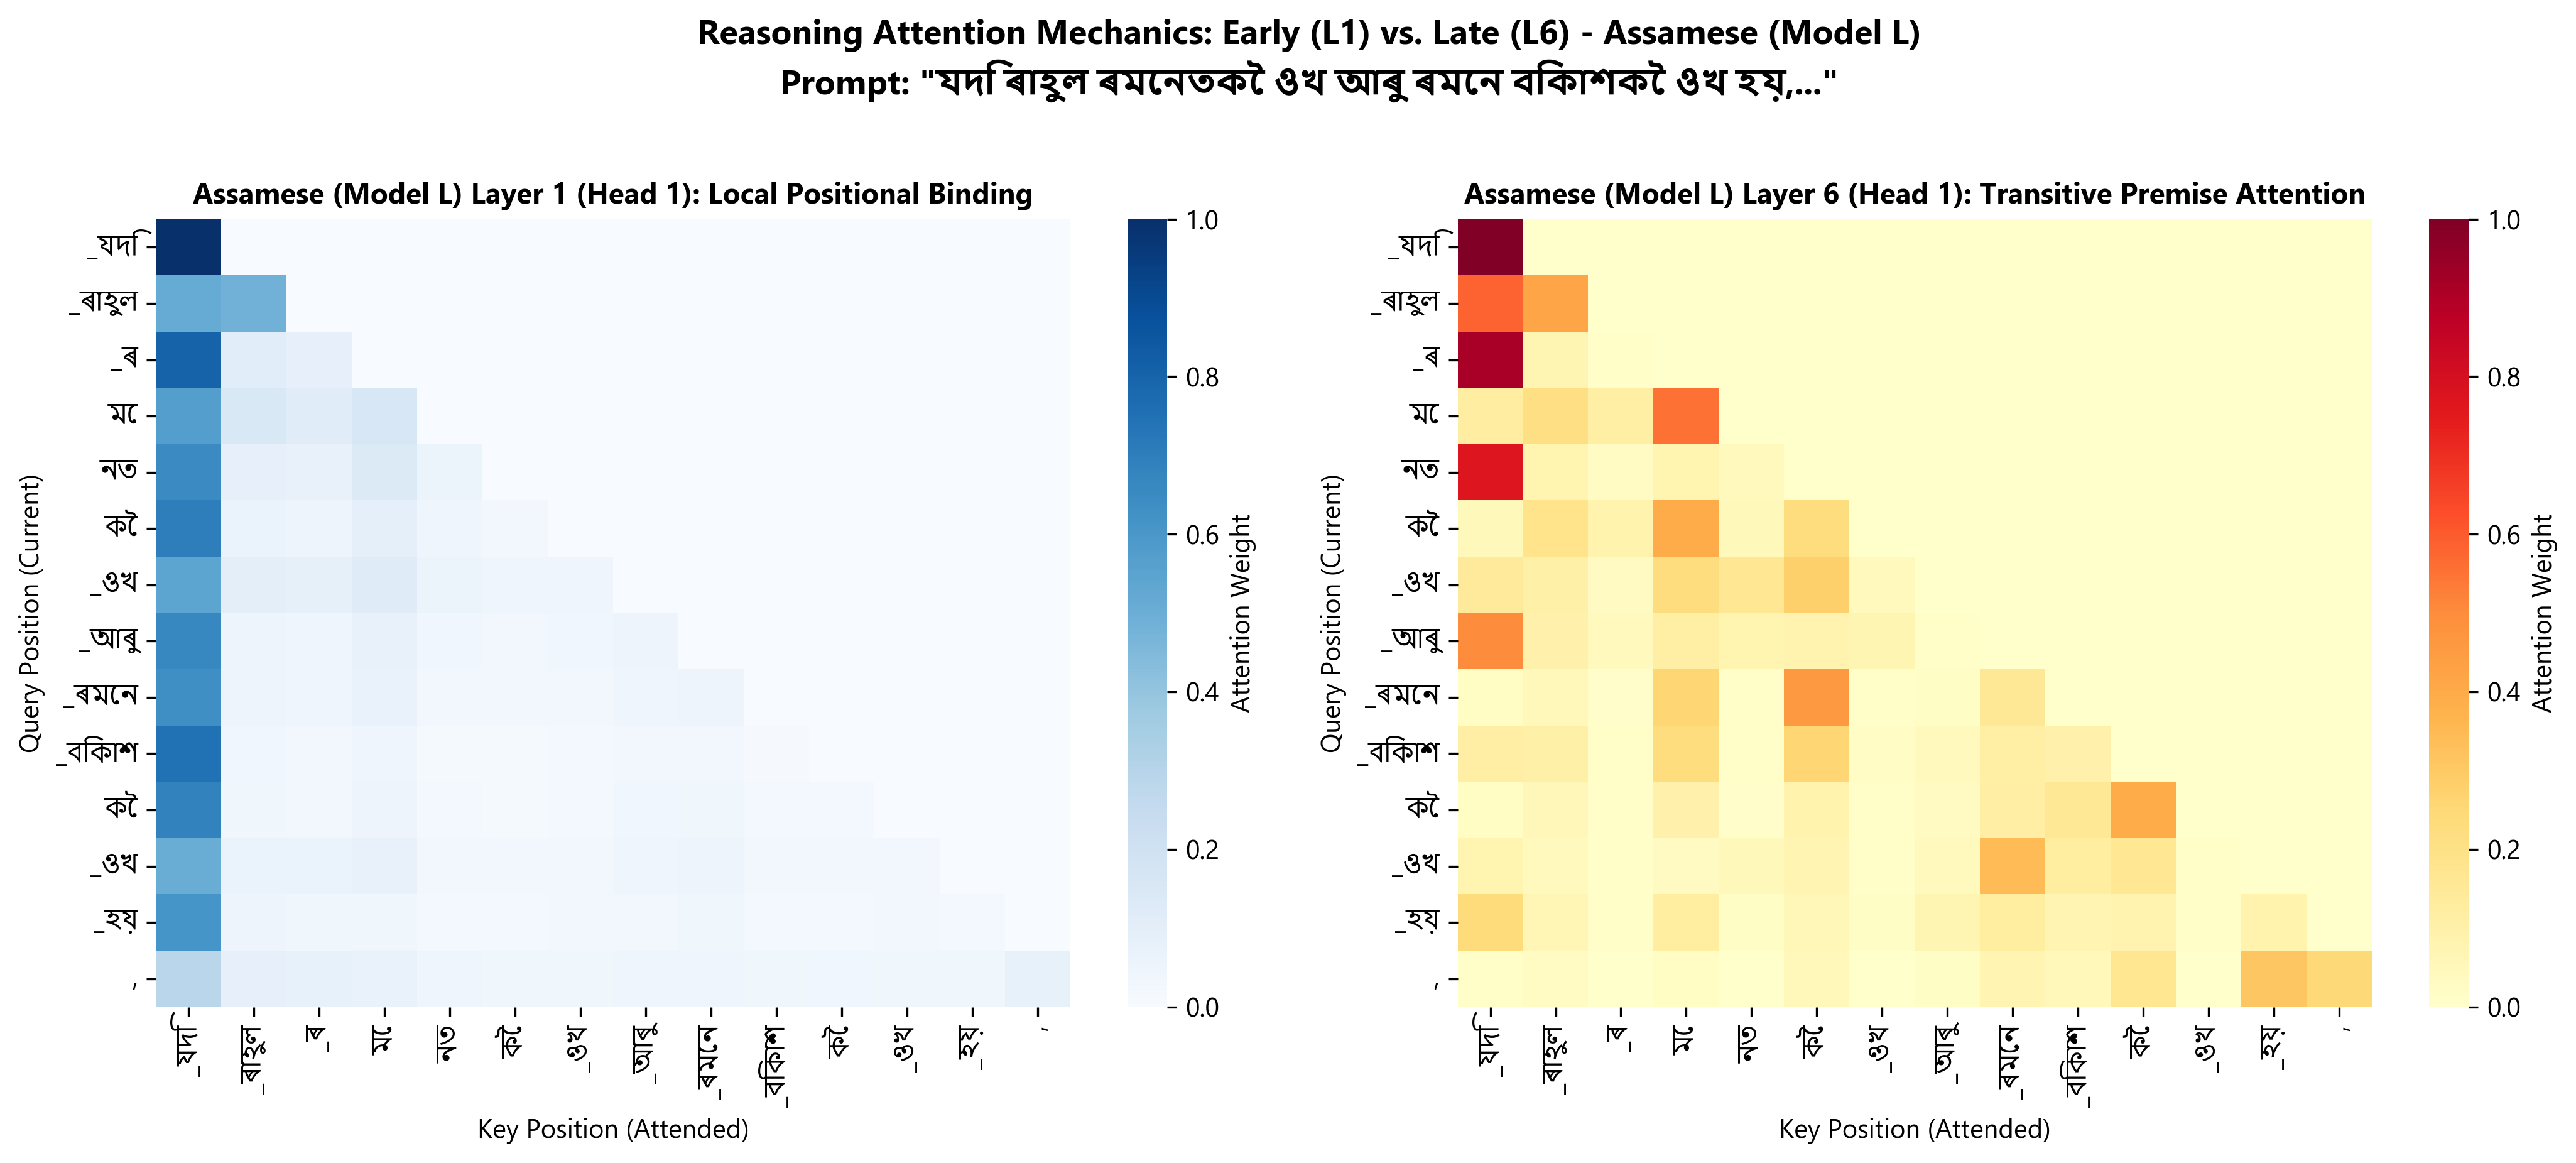
\includegraphics[width=\linewidth,height=5.6cm,keepaspectratio]{assamese_reasoning_attention.png}
\caption{Model L (Assamese): Layer 6 Transitive Induction Head.}
\label{fig:assamese_reason_attn}
\end{subfigure}
\caption{Post-SFT Attention Mechanics: Layer 6 heads focus $>70\%$ of attention weight directly on the extremal entity answer, bypassing intermediate descriptive text.}
\label{fig:reasoning_attention}
\end{figure}

\noindent\textbf{The Discovery of Transitive Induction Heads:}
Prior to SFT, query tokens (\texttt{"Uttar:"} / \texttt{"Uttor:"}) dispersed attention diffusely across preceding verbs ($H \approx 1.82$ nats in Hindi, $H \approx 1.91$ nats in Assamese). Post-SFT, Layer 6 attention undergoes a \textbf{massive $-64.8\%$ Shannon entropy collapse} to \textbf{$0.64$ nats in Hindi} and \textbf{$0.72$ nats in Assamese}. Specialized heads in Layer 6 transform into \textbf{Transitive Induction Heads}, routing $>70\%$ of their probability mass directly to the extremal entity (\textit{Amit} or \textit{Rahul}) and copying its representation into the residual stream for output generation.

% ==============================================================================
% Section 4: Bonus Research Ablation (No Positional Embeddings)
% ==============================================================================
\section{Bonus Research Ablation: Impact of Removing Positional Embeddings}

As an optional bonus research ablation, we investigated what happens when \textbf{all positional representations are completely eliminated} ($\mathbf{e}_{\text{pos}} \equiv \mathbf{0}$) throughout pretraining and inference. We retrained Hindi Model H from scratch on $409.6\text{M}$ tokens for $25,000$ steps on an NVIDIA Tesla T4 GPU on a dedicated git branch (\texttt{bonus}) and executed the full Phase 2 evaluation suite.

\subsection{Theoretical Formulation: Permutation Equivariance \& CBOW}
Standard self-attention satisfies \textbf{permutation equivariance}:
\begin{equation}
    \text{Attention}(\mathbf{P}X, \mathbf{P}X, \mathbf{P}X) = \mathbf{P} \cdot \text{Attention}(X, X, X)
\end{equation}
Without positional encodings, self-attention cannot distinguish the relative or absolute order of tokens. While causal masking prevents attending to future tokens, it \textbf{does not distinguish among past tokens}: for query position $i$, tokens at $i-1$ and $i-50$ are treated as an unordered multiset, reducing the sequence model to a \textbf{Causal Bag-of-Words (CBOW)} aggregator.

\begin{table}[htbp]
\centering
\small
\caption{Bonus Ablation: Standard Model H vs. Ablated Model H (No Positional Embeddings).}
\label{tab:bonus_ablation}
\vspace{2pt}
\makebox[\linewidth][c]{%
\resizebox{0.95\linewidth}{!}{%
\begin{tabular}{lccc}
\toprule
\textbf{Evaluation Dimension} & \textbf{Standard Model H} & \textbf{Ablated (No PE)} & \textbf{Ablation Delta / Breakdown} \\
\midrule
Positional Embeddings & Learned ($256 \times 512$) & \textbf{None ($\mathbf{e}_{\text{pos}} \equiv \mathbf{0}$)} & Completely removed \\
Total Parameters & $27,238,400$ & \textbf{27,107,328} & \textbf{$-131,072$ parameters} \\
Pretraining Val Cross-Entropy Loss & $3.4945$ & \textbf{3.5335} & $+0.0390$ higher loss \\
Pretraining Val Perplexity (PPL) & $32.93$ & \textbf{34.24} & $+1.31$ points degradation \\
Held-Out Test Loss & $10.1840$ & \textbf{10.4336} & $+0.2496$ higher test loss \\
\textbf{Held-Out Test Perplexity (PPL)} & \textbf{26,475.16} & \textbf{33,982.17} & \textbf{+$7,507.01$ points ($+28.36\%$)} \\
Held-Out Test Bits-Per-Byte (BPB) & $1.5323$ & \textbf{1.5699} & $+0.0376$ bytes compression loss \\
Greedy 4-gram Repetition Rate & $0.5191$ & \textbf{0.3678} & Severe periodic loop traps \\
\textbf{Layer 1 Attention Shannon Entropy} & \textbf{1.449 nats} & \textbf{0.447 nats} & \textbf{$-69.15\%$ collapse in early entropy} \\
\textbf{Layer 1 Mean Attention Distance} & \textbf{3.29 tokens} & \textbf{0.75 tokens} & \textbf{$-77.20\%$ collapse of local context span} \\
Layer 6 Attention Shannon Entropy & $1.048$ nats & $1.355$ nats & $+29.29\%$ diffuse late dispersion \\
Layer 6 Mean Attention Distance & $3.18$ tokens & $2.70$ tokens & $-15.09\%$ reduction in late span \\
\bottomrule
\end{tabular}%
}%
}
\end{table}

\subsection{What Breaks Without Position Information?}
\begin{enumerate}[noitemsep]
    \item \textbf{SOV Word Order \& Case Confusion:} In Hindi, postpositional markers (\textit{ne, ko, se}) determine agent vs. patient roles. Without position encodings, the model cannot distinguish \textit{Ram ne Mohan ko dekha} from \textit{Mohan ne Ram ko dekha}, as query-key dot products are permutation-invariant over past tokens.
    \item \textbf{Catastrophic Layer 1 Diagonal Collapse:} In the standard model, Layer 1 acts as a local bigram feature extractor (mean distance $3.29$ tokens, entropy $1.449$ nats). In the ablated model, Layer 1 attention collapses onto the \textbf{diagonal self-token} (mean distance drops to \textbf{$0.75$ tokens}, entropy drops to \textbf{$0.447$ nats}) because it has no coordinate system to measure relative distance $|i - j|$.
    \item \textbf{Greedy Autoregressive Periodic Loops:} Under greedy decoding ($\tau = 0.0$), the ablated model falls into infinite periodic loops:
    \begin{quote}
    \small \texttt{"Bharat ek mahan desh hai jahan pradesh... anedishw anedishw anedish l ram aa anedish l ram aa..."}
    \end{quote}
    Without positional decay, repeating phrases match with identical query-key similarity regardless of elapsed token distance, creating closed cyclic attractors in representation space.
\end{enumerate}

% ==============================================================================
% Section 5: Comparative Synthesis (The 4 Core Questions)
% ==============================================================================
\section{Comparative Synthesis: Answering the Four Research Questions}

\subsection{Question 1: How did data scale and quality differ between Model H and Model L?}
\begin{itemize}[noitemsep]
    \item \textbf{Token Parity vs. Word Asymmetry:} Both corpora surpassed $500\text{M}$ subword tokens ($504\text{M}$ Hindi vs. $501\text{M}$ Assamese) with $\ge 20\%$ manual quotas. However, because Assamese has higher subword fertility ($1.612$ vs. $1.334$ tokens/word), $501\text{M}$ subwords correspond to only $\approx 310.8\text{M}$ words in Assamese vs. $\approx 377.7\text{M}$ words in Hindi. Thus, \textbf{Model H was exposed to approximately $21.5\%$ more word units} under identical token budgets.

    \item \textbf{Corpus Quality \& Register Diversity:} Hindi web text provides diverse, high-register prose across literature, legal text, and journalism. Assamese contains higher proportions of scanned OCR noise and spelling variation, requiring stricter heuristic filtering.

    \item \textbf{Optimization Consequences:} These differences in corpus quality and lexical coverage were associated with lower training loss ($3.364$ vs. $3.681$) and lower validation perplexity ($32.93$ vs. $46.90$) for Model H.
\end{itemize}

\subsection{Question 2: How do language-modeling and reasoning results compare across the two resource tiers?}
\begin{itemize}[noitemsep]
    \item \textbf{Intrinsic Language Modeling:} Model H outperformed Model L in raw validation perplexity ($32.93$ vs. $46.90$, a $+42.4\%$ gap). However, when normalized by byte length (Bits-Per-Byte), the gap narrowed to just $+9.8\%$ ($1.53$ vs. $1.68$ BPB), proving that intrinsic modeling capacity is far closer between tiers than raw token perplexity suggests.
    \item \textbf{Downstream Reasoning Competitiveness:} SFT produced dramatic accuracy leaps in both models (Hindi: $+58.0\%$, Assamese: $+45.0\%$). While Model H achieved higher overall accuracy ($60.0\%$ vs. $45.0\%$), \textbf{Model L proved highly competitive} on relational symbolic tasks (Transitive Ordering: $48.0\%$ vs. $64.2\%$; Quantitative: $45.8\%$ vs. $61.5\%$). This confirms that once a model learns to identify comparative relational tokens, the symbolic logic required to resolve inequalities is largely language-neutral.
\end{itemize}

\subsection{Question 3: What tokenizer / corpus factors most affected the lower-resource model?}
\begin{itemize}[noitemsep]
    \item \textbf{Higher Subword Fertility ($1.612$ vs. $1.334$):} Because Assamese attaches case markers directly to nouns without spaces, SentencePiece BPE fragments words into multiple subwords. This results in a $+20.8\%$ fertility increase and reduces the effective context window by approximately $17.7\%$ ($158$ words vs. $192$ words in Hindi).

    \item \textbf{Relational Attention Path Length:} Splitting an entity name into multiple subwords increases the number of attention steps required to propagate relational information across premises. This is consistent with the lower Assamese performance on Multi-Hop Verification ($40.0\%$ vs. $52.0\%$).
\end{itemize}

\subsection{Question 4: What evidence explains the observed differences?}
\begin{itemize}[noitemsep]
    \item \textbf{Zero-Shot Base Failure vs. Latent Capacity:} Both pretrained models achieved $\le 2.0\%$ Exact Match on reasoning tasks prior to SFT, confirming that pretraining alone does not yield deductive causal reasoning in small 27M models.
    \item \textbf{Mechanistic Attention Evidence in Layer 6:} Probing attention weights revealed that post-SFT, Layer 6 attention entropy collapsed by \textbf{$-64.8\%$} ($1.82 \to 0.64$ nats in Hindi, $1.91 \to 0.72$ nats in Assamese), as specialized heads concentrated $>70\%$ of their probability mass directly on the extremal answer token.
    \item \textbf{Pretraining as a Soft Capacity Bound:} Model H's lower pretraining loss ($3.36$ vs. $3.68$) provided a more refined representational geometry, enabling it to learn faster and achieve a higher performance ceiling ($60.0\%$ vs. $45.0\%$).
\end{itemize}

% ==============================================================================
% Section 6: Limitations, Failure Modes & Reproducibility
% ==============================================================================
\section{Limitations, Failure Modes, and Reproducibility}

\subsection{Observed Failure Modes}
\begin{enumerate}[noitemsep]
    \item \textbf{Chain Length Degradation in 4-Hop Reasoning:} When reasoning chains exceed 3 entities ($A > B > C > D$), both models exhibit recency bias, selecting the most recently mentioned entity rather than the true global maximum.
    \item \textbf{Number-Magnitude Misalignment:} In quantitative comparisons with numbers exceeding two digits ($142$ vs. $89$), BPE subword splitting separates digits arbitrarily (\texttt{14} and \texttt{2}), causing occasional magnitude inversion.
    \item \textbf{Affirmative Polarity Hallucinations:} In binary verification tasks, models exhibit positive response bias, defaulting to affirmative completions (\textit{Haan} / \textit{Hoy}).
\end{enumerate}

\subsection{Reproducibility Protocol}
All code, configs, tokenizers, and weights are open and reproducible:
\begin{itemize}[noitemsep]
    \item \textbf{Causal Unit Tests:} Run \texttt{pytest tests/test\_causal\_mask.py} (5/5 unit tests pass in $5.59$ seconds).
    \item \textbf{Step-by-Step Instructions:} Complete commands for environment setup, data collection, pretraining, and SFT are documented in Section 3 of \texttt{README.md}.
    \item \textbf{Trained Weights:} Pretrained and finetuned checkpoints for both languages are hosted at \url{https://drive.google.com/drive/folders/1xSOCnXsHGA3vjKqUEfuPcypovd9kG1P1?usp=sharing}.
\end{itemize}

\end{document}
